% **************************************************
% Document Class Definition
% **************************************************
\documentclass[%
    paper=A4,               % paper size --> A4 is default in Germany
    twoside=true,           % onesite or twoside printing
    openright,              % doublepage cleaning ends up right side
    parskip=full,           % spacing value / method for paragraphs
    chapterprefix=true,     % prefix for chapter marks
    11pt,                   % font size
    headings=normal,        % size of headings
    bibliography=totoc,     % include bib in toc
    listof=totoc,           % include listof entries in toc
    titlepage=on,           % own page for each title page
    captions=tableabove,    % display table captions above the float env
    draft=false,            % value for draft version
]{scrreprt}%


% **************************************************
% Setup YOUR thesis document in this file !
% **************************************************
% !TEX root = main.tex


% **************************************************
% Files' Character Encoding
% **************************************************
\PassOptionsToPackage{utf8}{inputenc}
\usepackage{inputenc}


% **************************************************
% Information and Commands for Reuse
% **************************************************
\newcommand{\thesisTitle}{Optimizer Ensembles for Automated Machine Learning}
\newcommand{\thesisName}{Lukas Brandt}
\newcommand{\thesisMatNr}{7011823}
\newcommand{\thesisSubject}{Master’s Thesis}
\newcommand{\thesisDate}{\today}

\newcommand{\thesisFirstReviewer}{Prof. Dr. Eyke Hüllermeier}
\newcommand{\thesisFirstReviewerUniversity}{\protect{Paderborn University}}
\newcommand{\thesisFirstReviewerDepartment}{Intelligent Systems and Machine Learning Group (ISG)}

\newcommand{\thesisSecondReviewer}{Jun. Prof. Dr. Henning Wachsmuth}
\newcommand{\thesisSecondReviewerUniversity}{\protect{Paderborn University}}
\newcommand{\thesisSecondReviewerDepartment}{Computational Social Science Group (CSS)}

\newcommand{\thesisFirstSupervisor}{Marcel Mever}

\newcommand{\thesisUniversity}{Paderborn University}
\newcommand{\thesisUniversityDepartment}{Department of Electrical Engineering, Computer Science and Mathematics}
\newcommand{\thesisUniversityInstitute}{Heinz Nixdorf Institute}
\newcommand{\thesisUniversityGroup}{Intelligent Systems and Machine Learning Group (ISG)}
\newcommand{\thesisUniversityStreetAddress}{Warburger Straße 100}
\newcommand{\thesisUniversityPostalCode}{33098}
\newcommand{\thesisUniversityCity}{Paderborn}



% **************************************************
% Debug LaTeX Information
% **************************************************
%\listfiles


% **************************************************
% Load and Configure Packages
% **************************************************
\usepackage[english]{babel} % babel system, adjust the language of the content
\PassOptionsToPackage{% setup clean thesis style
    figuresep=colon,%
    sansserif=false,%
    hangfigurecaption=false,%
    hangsection=true,%
    hangsubsection=true,%
    colorize=full,%
    colortheme=upbisg,%
    bibsys=biber,%
    bibfile=bib-refs,%
    bibstyle=alphabetic,%
    wrapfooter=false,%
}{cleanthesis}
\usepackage{cleanthesis}

\usepackage{mathtools}

\usepackage[font=sf]{caption}

\usepackage{amssymb}

\usepackage{subcaption}

\usepackage{listings}

\usepackage{dirtree}

\usepackage{fancyvrb}

\usepackage{booktabs}

\usepackage[figuresright]{rotating}

\usepackage[linesnumbered,ruled,vlined]{algorithm2e}

\usepackage{pgfplots}
\pgfplotsset{colormap/viridis}

%TikZ Setup
\usepackage{tikz}
\usetikzlibrary{fit}

\hypersetup{% setup the hyperref-package options
    pdftitle={\thesisTitle},    %   - title (PDF meta)
    pdfsubject={\thesisSubject},%   - subject (PDF meta)
    pdfauthor={\thesisName},    %   - author (PDF meta)
    plainpages=false,           %   -
    colorlinks=false,           %   - colorize links?
    pdfborder={0 0 0},          %   -
    breaklinks=true,            %   - allow line break inside links
    bookmarksnumbered=true,     %
    bookmarksopen=true          %
}



% **************************************************
% Document CONTENT
% **************************************************
\begin{document}

% --------------------------
% rename document parts
% --------------------------
%\renewcaptionname{ngerman}{\figurename}{Abb.}
%\renewcaptionname{ngerman}{\tablename}{Tab.}
\renewcaptionname{english}{\figurename}{Fig.}
\renewcaptionname{english}{\tablename}{Tab.}

% --------------------------
% Front matter
% --------------------------
\pagenumbering{roman}			% roman page numbing (invisible for empty page style)
\pagestyle{empty}				% no header or footers
% !TEX root = ../main.tex
%
% ------------------------------------  --> cover title page
\begin{titlepage}
	\pdfbookmark[0]{Cover}{Cover}
	\flushright
	\hfill
	\vfill
	{\LARGE\thesisTitle \par}
	\rule[5pt]{\textwidth}{.4pt} \par
	{\Large\thesisName}
	\vfill
	\textit{\large\thesisDate}
\end{titlepage}


% ------------------------------------  --> main title page
\begin{titlepage}
	\pdfbookmark[0]{Titlepage}{Titlepage}
	\tgherosfont
	
	\begin{figure}
	\begin{minipage}[t]{8.5cm}		
	
\includegraphics[height=1.8cm]{gfx/upb_1E}\\
	\textsf{\small{\hspace*{1.3cm}Department of Electrical Engineering,\\
	\hspace*{1.3cm}Computer Science and Mathematics\\
%		\hspace*{1.3cm}Institute of Computer Science\\
		\hspace*{1.3cm}Warburger Straße 100 \\
		\hspace*{1.3cm}33098 Paderborn
		}}
	\end{minipage}
	\hfill
	\begin{minipage}[t]{4.7cm}
	
\includegraphics[height=1.8cm]{gfx/is-logo-klein}\\
	\textsf{%Institute of Computer Science\\
	\hspace*{0.1cm}\small{Intelligent Systems Group (ISG)}
	}
	\end{minipage}
	\end{figure}
	
	\centering
	%\textsf{\thesisUniversityDepartment} \\
	%\textsf{\thesisUniversityGroup} \\

	\vfill
	{\large \thesisSubject} \\[5mm]
	{\LARGE \color{ctcolortitle}\textbf{\thesisTitle} \\[10mm]}
	{\Large \thesisName} \\

	\vfill
	\begin{minipage}[t]{.27\textwidth}
		\raggedleft
		\textit{1. Reviewer}
	\end{minipage}
	\hspace*{15pt}
	\begin{minipage}[t]{.65\textwidth}
		{\Large \thesisFirstReviewer} \\
	  	{\small \thesisFirstReviewerDepartment} \\[-1mm]
		{\small \thesisFirstReviewerUniversity}
	\end{minipage} \\[5mm]
	\begin{minipage}[t]{.27\textwidth}
		\raggedleft
		\textit{2. Reviewer}
	\end{minipage}
	\hspace*{15pt}
	\begin{minipage}[t]{.65\textwidth}
		{\Large \thesisSecondReviewer} \\
	  	{\small \thesisSecondReviewerDepartment} \\[-1mm]
		{\small \thesisSecondReviewerUniversity}
	\end{minipage} \\[10mm]
	\begin{minipage}[t]{.27\textwidth}
		\raggedleft
		\textit{Supervisors}
	\end{minipage}
	\hspace*{15pt}
	\begin{minipage}[t]{.65\textwidth}
		\thesisFirstSupervisor
	\end{minipage} \\[10mm]

	\thesisDate \\

\end{titlepage}


% ------------------------------------  --> lower title back for single page layout
\hfill
\vfill
{
	\small
	\textbf{\thesisName} \\
	\textit{\thesisTitle} \\
	\thesisSubject, \thesisDate \\
	Reviewers: \thesisFirstReviewer\ and \thesisSecondReviewer \\
	Supervisors: \thesisFirstSupervisor \\[1.5em]
	\textbf{\thesisUniversity} \\
	\textit{\thesisUniversityGroup} \\
	\thesisUniversityInstitute \\
	\thesisUniversityDepartment \\
	\thesisUniversityStreetAddress \\
	\thesisUniversityPostalCode\ and \thesisUniversityCity
}
		% INCLUDE: all titlepages
\cleardoublepage

\pagestyle{plain}				% display just page numbers
% !TEX root = ../my-thesis.tex
%
\pdfbookmark[0]{Abstract}{Abstract}
\chapter*{Abstract}
\label{sec:abstract}
\vspace*{-10mm}

\blindtext

\vspace*{20mm}

{\usekomafont{chapter}Zusammenfassung}\label{sec:abstract-ger} \\

\blindtext
		% INCLUDE: the abstracts (english and german)
\cleardoublepage
%
% !TEX root = ../my-thesis.tex
%
\pdfbookmark[0]{Acknowledgement}{Acknowledgement}
\chapter*{Acknowledgement}
\label{sec:acknowledgement}
\vspace*{-10mm}

\Blindtext[2][2]
 % INCLUDE: acknowledgement
\cleardoublepage
%
\setcounter{tocdepth}{2}		% define depth of toc
\tableofcontents				% display table of contents
\cleardoublepage

% --------------------------
% Body matter
% --------------------------
\pagenumbering{arabic}			% arabic page numbering
\setcounter{page}{1}			% set page counter
\pagestyle{maincontentstyle} 	% fancy header and footer

% !TEX root = ../my-thesis.tex
%
\chapter{Introduction}
\label{sec:intro}

\section{Motivation}
\label{sec:intro:motivation}

Since machine learning is present in a fast growing part of everyday life, economy and science, the number of people who want to use machine learning and apply it to their use case is equally fast growing.
The problem is that using machine learning beyond simple examples and tutorials requires theoretical domain knowledge as well as solid programming skills.\newline
Applying a machine learning approach includes the selection of a suitable learning model or even multiple models and other components combined to a complex pipeline.
The cautious choice of machine learning algorithms for each problem or use-case is crucial to have a suitable and well performing pipeline.
Each selected machine learning algorithm may expose hyperparameters in return and the configuration of these parameters is a second necessary step for the application of machine learning.
Finally, the selected model or pipeline with the configured parameters must be actually implemented with a suitable programming language within a machine learning framework or toolbox, which are usually comparably big and complex individual parts.
Therefore, caused by these three necessary steps there is a learning and knowledge barrier that prevents interested people with a non-technical background from using machine learning.

In the last years, different approaches were developed, which can take this barrier off their shoulders and empower nearly everyone to use machine learning for datasets of their domain or setting.
These approaches allow this by automating this algorithm configuration problem, consisting of the described sub-problems: Selecting models (respectively components of pipelines), configuring all required parameters and constructing a usable implementation.
All the end-user has to do is to provide their data in a suitable dataset format and usually specify a resource or time budget for the solver of the algorithm configuration problem.\newline
Within this budget, the best pipeline can be searched regarding a metric, as for example the predictive accuracy.
Hence, this problem of finding a machine learning pipeline for a dataset can be considered an optimization problem.
Solving this optimization problem is the challenge of a research area called \textit{Automated Machine Learning} or short \textit{AutoML}.

AutoML received much attention in the scientific machine learning community and a broad spectrum of different methods were developed and published.
The majority of these approaches and the plethora of different strategies they utilize, have usually one thing in common.
They see the model selection and the model configuration as a joint optimization problem and therewith solve this two problems within a single optimization space with a single optimization algorithm.\newline
However, recently a few new approaches were published that split this joint optimization space and utilize different optimization methods for the two respective spaces.
But this application of more than one optimization algorithm can be extended to three or more optimizers and in theory, this should show an improvement because of the \textit{No-free-lunch Theorems for optimization}.
It states that when an optimization algorithm performs under constraints superior for one problem or class of problems it has to pay for this by performing inferior for other problems.
In the context of AutoML this would imply that one optimization approach, can not yield the best solution across all datasets, timeouts, and pipeline component domains.

Combining multiple optimization methods into an ensemble of optimizers would allow this ensemble to optimize each possible pipeline with the most suitable optimization algorithm with respect to the parameter space of this pipeline and the properties of the dataset.
Therewith, the most suitable optimization algorithm out of the ensemble could be identified and exploited to the given AutoML problem setting.\newline
For creating and utilizing this optimizer ensembles in the context of AutoML, a novel approach is required and will be the topic of this thesis. 

\section{Thesis Goal and Research Questions}
\label{sec:intro:goal}
In the context of this thesis, a feasible concept and algorithm for such optimizer ensembles will be devised and exemplarily realized as a reference implementation.
This  implemented optimizer ensemble algorithm will be the test subject for a series of empirical evaluations.\newline
Overall, the goal of this thesis is to answer two research questions regarding this approach for optimizer ensembles in the focus of AutoML with the data gathered during the evaluations:
\begin{enumerate}
    \item Is the devised approach for optimizer ensembles feasible in the context of AutoML?
    More precisely, is the result quality comparable or even better compared to other state-of-the-art approaches?
    And if it is a feasible approach, what influence have the particular components of the approach on the overall outcome?
    \item Can knowledge about the optimization in the general AutoML context be extrapolated from this approach?
    When the frequencies of utilizing certain optimizations algorithms during the execution of this approach are recorded, this may give indications regarding their capability for different AutoML problems, since this approach tries to find the best suited optimizer out of the ensemble for the input problem and exploit it.
    Based on this frequencies, is every optimizer called an equal amount of times or is one or more optimization method favoured for the AutoML use case?
    Does it depend on certain dataset properties of the concrete AutoML problem, whether an optimization method is used relatively often?
\end{enumerate}

\section{Thesis Structure}
\label{sec:intro:structure}
Following this introduction, this thesis is structured into five chapters.
The content and goals of each chapter are briefly explained here:

\textbf{Chapter \ref{sec:theory}} \\[0.2em]
At first, the foundations of the machine learning, the AutoML setting and optimization in general are elucidated, to give a starting point for the related work part of this chapter and aid the understanding of the approach of this thesis.
A selection of Black Box optimization algorithms is presented and for each one a few existing AutoML approaches, which apply this specific optimization algorithm, as well.\newline
With the help of the No-Free-Lunch theorems for optimization, it will be argued why it is not sufficient to utilize a single optimization method for a single AutoML optimization space.\newline
The chapter is concluded by presenting a few recently published AutoML approaches, which already apply the idea of separating the single joint optimization space and applying more than one optimizer, as supplementary related works besides the AutoML approaches, which were presented priorly in this chapter altogether with their utilized black box optimization algorithm.

\textbf{Chapter \ref{sec:approach}} \\[0.2em]
The optimizer ensemble approach of this thesis is theoretically specified here and the underlying design choices explained and justified.
Every concept mentioned in the theory chapter, which is taken up again for the specification of this approach, is explained in more detail here as well.\newline
All improvements from applying an optimizer ensemble instead of a single optimizer are listed with reference to the disadvantages from the related work approaches mentioned in chapter~\ref{sec:theory}.

\textbf{Chapter \ref{sec:implementation}} \\[0.2em]
To apply the approach for actual AutoML problem settings as well as evaluating the approach empirically in an experiment series, an actual implementation is necessary.
The technical details of an exemplaric reference implementation as a tool developed with the Python programming language are explicated in this chapter, accompanied with an overview of the utilized libraries of the implementation.

\textbf{Chapter \ref{sec:evaluation}} \\[0.2em]
In order to answer the previously listed research questions, a series of empirical experiments is designed and conducted.\newline
This approach is benchmarked against state-of-the-art scores of some of the related work approaches as well as altered versions of itself.
Structured by the addressed research question, the experiments design and execution is explained.
Subsequent to this explanations, the results of the experiments are shown and interpreted to answer the research questions.

\textbf{Chapter \ref{sec:conclusion}} \\[0.2em]
Finally, the answers to the research questions are used to summarize the concepts of this approach and their validity.
At last, an outlook is given about additions, which could further improve this approach and are a starting point for future work and follow-up research.

% !TEX root = ../my-thesis.tex
%
\chapter{Theoretical Foundations}
\label{sec:theory}
Before presenting the approach for tackling AutoML with an ensemble of optimizers, some theoretical foundations of both elements, AutoML and optimization, are given in the following.
This theoretical background is structured in three parts:
\begin{enumerate}
    \item Some basic concepts and intuitions of machine learning in general are outlined alongside with the challenges and problems that arise when applying machine learning.
    \item The concepts and usual approaches of AutoML are introduced, which were developed to tackle the listed challenges of classical machine learning. In addition, the connection between the AutoML setting and typical optimization problems is illustrated.
    \item As the foundation for building an ensemble of optimizers a selection of established optimization methods is given and explained.
\end{enumerate}
The overview of optimization methods is concluded with the discussion of a theoretical drawback of using a single optimization method.
Before explaining the ensemble approach, which could counter this drawback to a certain degree, in the next chapter, this discussion is continued with a selection of related works, where other approaches that addressed this theoretical disadvantage of using a single optimization method are mentioned. 

\section{Classical Machine Learning}
\label{sec:theory:ml}
If a human is given a task where the correct solution or reaction is not evident, a humans has always the possibility to react with a random solution or with an arbitrary reaction.
But if the human has any prior first- or second-hand experience with the same of a similar task, the human can choose the reaction based on the memories of different outcomes for different reactions for the more or less similar prior task.
With the high abstraction level and very symbolic nature of human thinking and memorization, it is comparably easy for humans to recognize even remote similarities between tasks.\newline
This is very challenging for a computer in contrast, because the models of tasks, experiences, and outcomes of reactions to tasks have to be readable and understandable for a machine, i.e. be in any kind of structured and consistent format.
This setting can be formalized as a combination of $T, P$ and $E$, where $T$ is a class of tasks, $P$ a performance measurement for solutions of a specific instances of the tasks class $T$ and $E$ is either given or collected experience, i.e. performance measurements for certain solutions in the context of specific task instance $t\in T$~\cite{Mitchell-MachineLearning}.\newline
Of course it is possible for a human programmer to manually specify the solution with the best performance measurement for any possible $t\in T$ but for a high $|T|$ this is rarely possible and viable.
Here, machine learning has its use-case: "Machine learning enables us to tackle tasks that are too difficult to solve with fixed programs written and designed by human beings"~\cite{Goodfellow-DeepLearning}.\newline
A high number of different types of task classes $T$ is imaginable, but one of the common one is \textit{Supervised Learning}.
In supervised learning, $T$ includes a fix set of all possible solutions $S$.
The concrete task for Supervised Learning is now to select for a given $t\in T$ a $s\subseteq S$ such that $P(t,s)$ is optimal.
To enable a machine to learn supervised, the experience $E$ has to be successively build in the form of $\{(t_1, s_1, P(t_1, s_1)), ..., (t_n, s_n, P(t_n s_n))\}$.
For a new task instance $t_i$, the computer will select a $s_i$ based on a decision model build from $E$, receive a performance feedback $P(t_i, s_i)$ and finally enrich $E$ with $(t_i, s_i, P(t_i, s_i))$ as well as updating the decision model with the changed $E$.
Therewith, a well working machine learning algorithm for supervised learning would now be able to achieve $P(t_j, s_j) \geq P(t_i, s_i)$ if $t_j$ and $t_i$ are similar instances, since it already has experience which $s\subseteq S$ had a certain performance value for $t_i$ and might therefore be a good or bad choice for $t_j$.\newline
This task of comparing and judging the similarity of different instances of $T$ and to build a practicable decision model based on $E$ to select a solution out of $S$ has been tackled with a plethora of different algorithms or even combinations of multiple algorithms as a form of machine learning pipeline.
Usually, this algorithms have to be configured with a set of hyperparameter depending on $T$ and often $T$ also has to be transformed before presenting concrete instances to the algorithm for learning, i.e. pre-processing each $t\in T$ with one or more transformation methods.
Without making suitable choices for the machine learning algorithm as well as corresponding hyperparameter and pre-processing methods for each different $T$, the performance measurements will only increase for a high $|E|$ or even not at all.
But because the number of available task instances, i.e. the amount of data, that can be used to build $E$ with a machine learning algorithm is often limited for most use-case domains, a valid choice for the learning algorithm, hyperparameter and, if necessary, pre-processing methods is crucial.\newline
With the high number of available machine learning algorithms and the often complex relationships between learning performance and hyperparameter configurations of the chosen algorithm as well as properties of $T$ and suitable pre-processing methods a big expertise in the machine learning field is necessary to be able to assemble machine learning applications with good performance measurements.
Since this necessary expertise in machine learning is not broadly available and a lot of companies or research facilities have a high demand for machine learning applications, it is not possible to apply machine learning in every use-case where it might be beneficial.
This accelerated the emergence of the machine learning research sub-topic \textit{Automated Machine Learning}. 

\section{Automated Machine Learning}
\label{sec:theory:automl}
Automated Machine Learning, or short \textit{AutoML}, tries to tackle this knowledge barrier, which prevents interested people from applying machine learning.
Therefore, the overall goal is to automate most tasks of the process of creating a machine learning application that would require machine learning knowledge.\newline
In this chapter at first a description of the general workflow of an AutoML tool is given and the usual two main steps of this workflow are illustrated.
This will be concluded with an formalization of the AutoML problem setting as an optimization problem.

\subsection{General Workflow}
\label{sec:theory:automl:workflow}
AutoML application are usually designed very homogeneous and therefore have very similar workflows among themselves.
As an input, the application will receive data in an machine-readable format and usually some form of constraint for its execution.
The expected outputs are the performance of the found machine learning pipeline regarding some task-dependent metric and the best found machine learning pipeline for the given data itself.
Additionally, each AutoML tool can have further configuration necessary as an input.\newline
The constraints for execution are required to prevent the AutoML tool from searching for the best machine learning pipeline for the given data indefinitely with probably continuously growing hardware consumption.
Therefore, the time and/or some hardware budgets are constrained.
This inputs and outputs of an conceptual AutoML tool are illustrated in figure~\ref{fig:theory:conceptualAutoMLTool}.\newline
\begin{figure}[ht!]
    \centering
    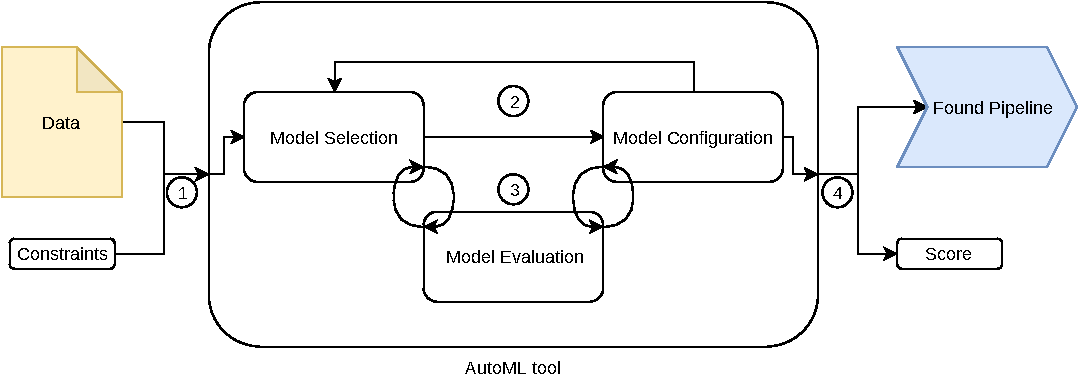
\includegraphics[width=\textwidth]{gfx/Figures/Theory/AutoMLTool.pdf}
    \caption{High level view of a conceptual AutoML tool. }
	\label{fig:theory:conceptualAutoMLTool}
\end{figure}
The general workflow of an AutoML tool is also numbered and illustrated in the figure and can be generalized with the following steps:
\begin{enumerate}
    \item AutoML tool gets input data and some execution constraints as an input.
    \item Model Selection and Model Configuration are repeated until execution constraints are met.
    \item Model Selection as well as Model Configuration can perform a Model Evaluation to get a score for any pipeline candidate they encounter.
    \item After the constraints are met, the best found pipeline as well as the score of this pipeline are given as an output.
\end{enumerate}
The Model Evaluation step is usually performed by training a pipeline on one big portion of the input data and testing it with a smaller portion of the data, sometimes called validation data, while measuring some kind of performance measurement, for example the accuracy of predictions or some error metric.
But other evaluation techniques for example like a Cross-Validation are also common.\newline
While the Model Evaluation step is only very loosely defined and usually not a complex procedure, the Model Selection and Model Configuration steps of the AutoML workflow are more sophisticated.
They have to select a suitable candidate from a usually large space. 
Both spaces, for Model Selection as well as for Model Configuration, will be individually explained in the following.

\subsection{Model Selection}
\label{sec:theory:automl:selection}
Model Selection is the task of selecting $1$ to $n$ components that will be part of the machine learning pipeline and sequentially traversed when data is passed through the pipeline.
For example, a valid pipeline would be to apply a Principal-Component-Analysis on the data as a first component and to use a Support Vector Machine for classification on the processed data as a second component afterwards.
In this step of the workflow, the space one candidate has to be selected from, consists of all this valid pipeline, which usually have two or more components.\newline
Usually there are three types of components:
\begin{itemize}
    \item Pre-Processing: Transform the input data before presenting it to the learning model.
    \item Learning Model: Perform the actual machine learning task on the data, for example classify a datapoint after training.
    \item Post-Processing: Transform the output of the learning model before yielding it as a final result.
\end{itemize}
Although in theory only a single learning model is necessary and components for pre- and post-processing are optional, at least pre-processing is very common in machine learning pipelines and included most of the time.\newline
It is possible to use more than one component from each type in a single pipeline and pipelines with arbitrary complexity can be created.
More than one pre- or post-processor can be used in sequence or in parallel with some kind of aggregator subsequently.
Equally, more than one learning model can be combined to be used as a composite model with a proper aggregation method like for example Bagging of models~\cite{Breiman-BaggingPredictors}.
An example for such a more complex pipeline is illustrated in figure~\ref{fig:theory:complexPipeline}.\newline
\begin{figure}[ht!]
    \centering
    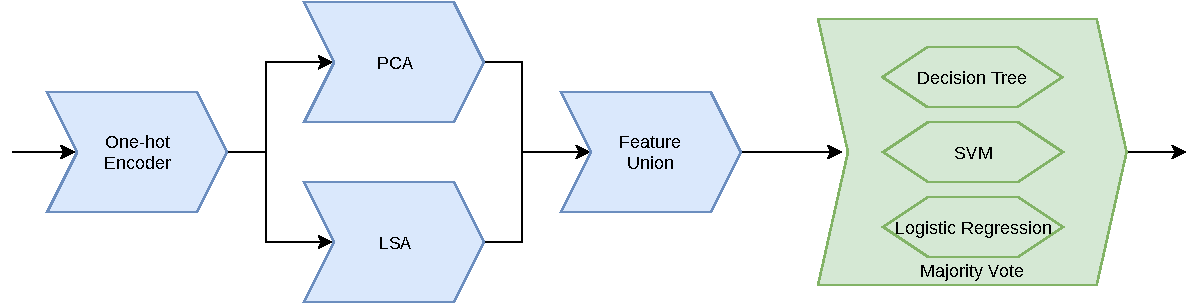
\includegraphics[width=\textwidth]{gfx/Figures/Theory/ComplexPipeline.pdf}
    \caption{Example for a more complex pipeline with four pre-processing components in blue: A One-hot Encoder, a Feature Union of a PCA and a LSA. The learning model in green is a Majority Voter as an aggregation of a Decision Tree, a SVM and a Logistic Regression Classifier. }
	\label{fig:theory:complexPipeline}
\end{figure}
Model Selection where the resulting pipelines can have this complexity needs to add a structural relationship between the pipeline components to the selected components.
Therewith, Model Selection can be written as simple formalization with two things:
\begin{itemize}
    \item For all possible components $C=\{c_1, ..., c_n\}$ a $C' \subseteq C$ of components that will be used to construct the pipeline.
    \item A binary relation $\prec$ over $C'$ that defines which component is a data input for another component to define an order of the components for the pipeline as well as aggregation of several components with one component. 
\end{itemize}
Nevertheless, to find a valid set $C' \subseteq C$ is not a trivial task.
For example, when an aggregator for multiple parallel pre-processing components is needed, a valid choice could be a Feature Union component but a Decision Tree component would be invalid for this pipeline position.
Therefore, if the pipelines shall be allowed to be more complex than for example a single pre-processing component and a single learning model, there is a big set of constraints for valid subsets of the candidate space of the Model selection $C$.

\subsection{Model Configuration}
\label{sec:theory:automl:configuration}
With the resulting component set after the Model Selection step selected its candidate $C'=\{c_1, ..., c_r\}$ the pipeline is not ready to be used yet.
Usually each component of $c_k \in C'$ has a set of hyperparameter and for each one a concrete value is needed.
Therewith, the candidate space for the Model Configuration step is dependent on the resulting candidate from the Model Selection step.
Each component $c_k$ has a set of hyperparameter $\Theta_k=\{ \theta_{k,1}, ..., \theta_{k,j} \}$ where each hyperparameter has a range where the value for this hyperparameter has to be chosen from.
Such a range can for example be a numeric set $\mathbb{N}$ or a custom set like for example $\{\textrm{true}, \textrm{false}\}$.\newline
When combining all ranges $\bigcup\limits_{i=1}^r \Theta_i$ a parametrization space with dimension $r$ is defined as the candidate space for the Model Configuration step, where configuration vectors can be drawn.
An example for a concrete parametrization drawn from a three dimensional parameter space is shown in figure~\ref{fig:theory:parameterSpace}
\begin{figure}[ht!]
    \centering
    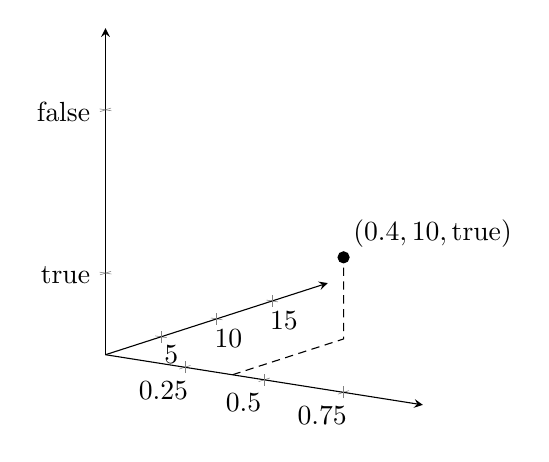
\begin{tikzpicture}
        \begin{axis}[
          view={35}{15},
          axis lines=center,
          xtick={0.25, 0.5, 0.75},ytick={5,10, 15},ztick={-10,-5,5,10},
          xmin=0,xmax=1,ymin=0,ymax=20,zmin=0.5,zmax=2.5,
          zticklabels={true, false},ztick={1,2},
          z tick label style={anchor=east}]
        ]
        \addplot3 [only marks] coordinates {(0.4,10,1)};
        \addplot3 [no marks,densely dashed] coordinates { (0.4,0,0.5) (0.4,10,0.5) (0.4,10,1)};
        \node [above right] at (axis cs:0.4,10,1) {$(0.4,10,\textrm{true})$};
        \end{axis}
    \end{tikzpicture}
    \caption{A parameter configuration with the values $(0.4,10,\textrm{true})$ inside the parameter space with the dimensions $[0..20]$, $[0, 1)$ and $\{\textrm{true}, \textrm{false}\}$ }
	\label{fig:theory:parameterSpace}
\end{figure}
Each of this vectors is a valid candidate and will result in a working pipeline instance created from $C'$ and configured with this vector.
When such a pipeline is constructed and configured with the vector values it can finally be evaluated as a candidate pipeline.

\subsection{Formalization of AutoML as an Optimization Problem}
\label{sec:theory:automl:optimization}
The choices in the Model Selection and Model Configuration step for one candidate out of the corresponding candidate spaces should not be arbitrary.
Evaluations of a candidate pipeline yield a score for this candidate and intuitively a suitable AutoML approach should try to select candidates with scores as good as possible.
Therefore, the AutoML problem is often considered as a special form of an optimization problem and can be formalized as one as well.\newline
\textcite{Feurer-Cash} give a formalization for AutoML problems as a so called \textit{Combined Algorithm Selection and Hyperparameter optimization} problem, or short \textit{CASH} problem.
Their definition is the following:
\begin{equation*}
    A^*, \lambda_* \in \> \underset{A^{(j)} \in \mathcal{A},\lambda \in \Lambda^{(j)}}{\mathrm{argmin}} \> \frac{1}{K} \sum_{i=0}^K \mathcal{L} (A_\lambda^{(j)}, D_{\textit{train}}^{(i)}, D_{\textit{valid}}^{(i)})
\end{equation*}
This formula consists out of the following parts:
\begin{itemize}
    \item $A^*$: The best solution of the algorithm selection, i.e. for the AutoML setting the best pipeline construction found in the Model Selection step
    \item $\lambda_*$: The best hyperparameter configuration for $A^*$ found in the hyperparameter optimization step, i.e. the Model Configuration step for AutoML
    \item $\mathcal{A}$: A set of possible algorithms to choose from and given in the form $\mathcal{A} = \{A^{1}, ..., A^{R} \}$, which is the set of all valid pipeline component combinations in the case of AutoML
    \item $\Lambda^{(j)}$: Each algorithm $A^{(j)} \in \mathcal{A}$ has a parameter configuration domain $\Lambda^{(j)}$, where a concrete parametrization $\lambda$ can be selected out of
    \item $\frac{1}{K} \sum_{i=0}^K $: This is used to calculate the K-fold cross-validation of a pipeline, but other evaluation metrics are also possible if the formula is adjusted accordingly
    \item $\mathcal{L} (A_\lambda^{(j)}, D_{\textit{train}}^{(i)}, D_{\textit{valid}}^{(i)})$: Is the loss, calculated with the loss function $\mathcal{L}$, of the algorithm $A^{(j)}$ configured with the parametrization $\lambda$, trained on the $i$-th split of the training data $D_{\textit{train}}^{(i)}$ and evaluated on the validation data $D_{\textit{valid}}^{(i)}$
\end{itemize}
In summary, the goal is to select an algorithm and a parameter configuration for this algorithm, such that the cross-validation loss for a for a given training and validation set is minimal.

\section{Black Box Optimization}
\label{sec:theory:optimization}
With the formalization of AutoML as a CASH problem the question arises if it can be tackled similar to standard textbook optimization problems, where established optimization algorithms exist.
Unfortunately, the CASH problem is a special case of optimization problem called \textit{Black Box} optimization problem.\newline
In the following will be explained in what way Black Box problems are different to the standard textbook optimization problem and why established optimization algorithms cannot be used.
Afterwards a selection of existing algorithms will be presented that can be used instead for the AutoML setting.
Finally, with the aid of the \textit{No-Free-Lunch Theorem}, it will be reasoned why these approaches cannot be optimal and why therefore a ensemble approach could be more promising.

\subsection{Differences to General Optimization Problems}
\label{sec:theory:optimization:differences}
\textcite{Boyd-Optimization} define a standard optimization problem as the following:
\begin{alignat*}{1}
    \underset{x}{\mathrm{minimize}} \textit{ or } \underset{x}{\mathrm{maximize}} \qquad & f_0(x)\\
    \textit{subject to} \qquad & f_i(x) \leq 0,\> i=1,...,m\\
                        &  h_j(x) \leq 0,\> j=1,...,p\\
\end{alignat*}
Here is the goal to find a value for the optimization variable $x$ such that $f_o(x)$ has either its minimum or maximum value.
Hereby, $x$ does not have to be a single value but can be a vector of values in the case of a multi-objective optimization problem.
$f_0$ is usually called a objective function or cost function.
The choices for $x$ can be limited by a set of inequality constraint functions $g_k$ and a set of equality constraint functions $h_i$.
If $m=p=0$, there are no constraint functions and the optimization problem is called unconstrained.
For such cases, x could be any value from the domain of $f_o$.\newline
If $f_0$ has certain properties, for example if it is convex, there are specialized optimization methods that can solve the optimization problem without the derivative $f_0'$.
But for general optimization algorithms, where no properties of $f_0$ besides derivability are expected, $f_0'$ is required to solve the optimization problem analytically.\newline
The problem is, for some optimization problems the exact formula of $f_0$ is not known or not given and therefore no derivative can be calculated such that the general optimization algorithms are not applicable.
Instead, it is only possible to obtain $f_0(x)$ for any requested $x$ for example by looking it up in a table or asking an expert.
For such problems it is only possible to observe the inputs and corresponding outputs of $f_0$ but the inner workings are hidden.
$f_0$ is metaphorically a black box, where something goes in and something comes out but it is not possible to look inside, and therefore such optimization problems are called Black Box optimization problems.\newline
AutoML, considered as a CASH problem, is a Black Box optimization problem as well.
It is not possible, or at least not yet realizable, to determine a general formula for $f_0$.
The relationship between the properties of the dataset, the different pipeline components with their configuration parameters and other factors, as for example randomness of some components, is way to complex and inscrutable to be formulated into a single cohesive function.
But it is possible to to get a evaluation of a $x$, i.e. a concrete pipeline with a complete configuration, by training and testing the pipeline with given data and a evaluation metric like for example a cross-validation.
The absence of a concrete formula for $f_0$ but the possibility to determine $f_0(x)$ renders AutoML as a Black Box optimization problem.\newline
Without the possibility to determine a optimal or near optimal candidate analytically, in the case of a Black Box optimization problem a series of candidates has to be selected and evaluated while trying to find or at least approximate a optimal solution.
Now the question remains for the AutoML setting how candidates from the two presumably large candidate spaces of Model Selection and Model Configuration should be selected for each iteration and how such a approximation can be attempted.\newline
A solely random selection in every iteration is not very likely to find good results with such a high number of choices.
Since the approach evaluates several candidates iteratively, a better approach would be to base the selection on knowledge gathered from previous iterations.\newline
Several algorithms were developed to tackle such a iteratively approximation of the optimum of a Black Box optimization problem.
Some of them have already showed promising results for AutoML CASH problems and therefore the current state-of-the-art AutoML research works primarily with the following three optimization strategies:
\begin{itemize}
    \item (Heuristic) Search
    \item Genetic and Evolutionary Algorithms
    \item Bayesian Optimization
\end{itemize}
In general is every Black Box optimization strategy defined by a selection of candidates out of the candidate space that will is evaluated and an order in which they are evaluated.
Hereby, the selection as well as the order can be defined in many ways.
For example it could be partially or fully pre-defined or random.
Also it could be defined implicitly and other selected candidates and their order can depend on the knowledge gathered from the evaluation of one candidate.\newline
For each one of the aforementioned Black-Box optimization strategies this candidate selection and candidate order will be explained in general and on the basis of some concrete algorithms, which were used in the AutoML research.
These explanations of the strategies will be supported with a simple running example.
The unconstrained target function $f_0 \left( \begin{bmatrix}x\\y \end{bmatrix} \right) = x^2 + y^2$, which can be seen in figure~\ref{fig:theory:target-function}, shall be minimized.
This function is defined in $\mathbb{R}^2$ and has one global minimum.
\begin{figure}[ht!]
    \centering
    \begin{subfigure}{0.48\textwidth}
        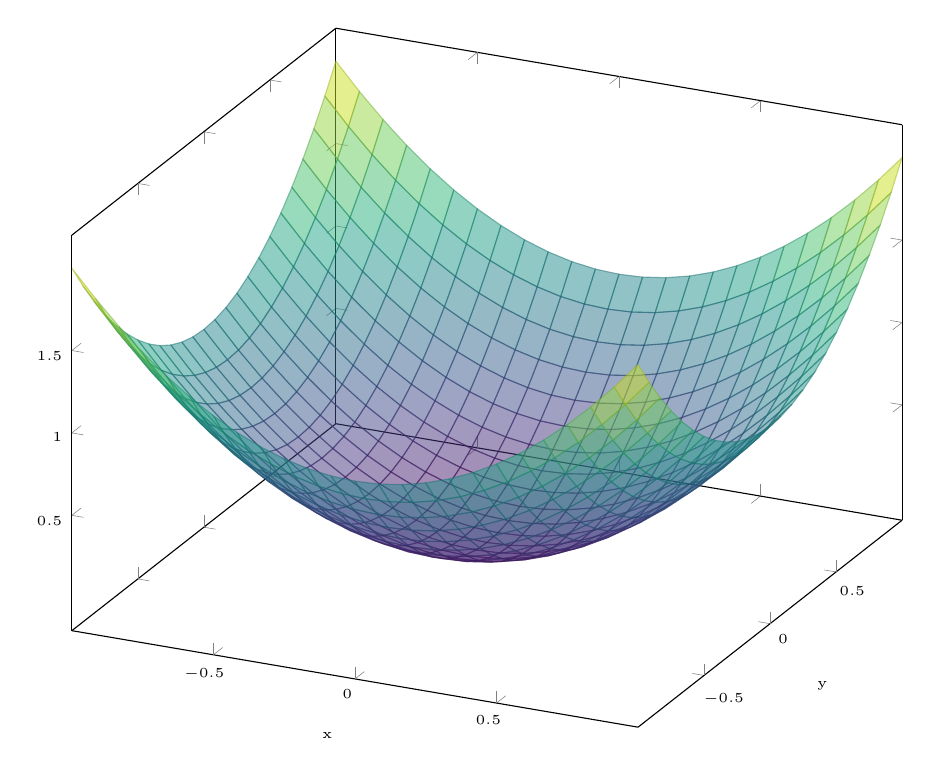
\begin{tikzpicture}
            \begin{axis}[
                xmin=-1,xmax=1,ymin=-1,ymax=1,
                width=\textwidth,
                xlabel = {x},
                ylabel = {y},
                xtick = {-0.5,0,0.5},
                ytick = {-0.5,0,0.5},
                ztick = {0.5,1,1.5},
                tick label style={font=\tiny},
                label style={font=\tiny}
            ]
                \addplot3[
                    surf,
                    opacity=0.5,
                    samples=25, samples y=25,
                    domain=-1:1, domain y=-1:1
                ]
                {x^2+y^2};
            \end{axis}
        \end{tikzpicture}
    \end{subfigure}
    \begin{subfigure}{0.48\textwidth}
        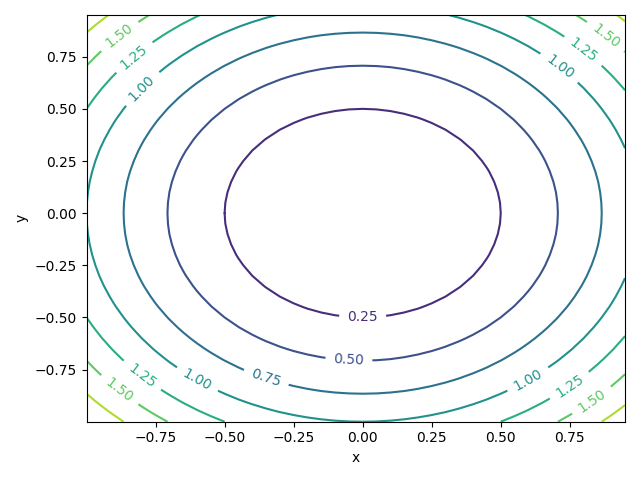
\includegraphics[width=\textwidth]{gfx/Figures/Theory/OptimizationTargetFunctionContour.png}
    \end{subfigure}
    \caption[.]{A two dimensional target function with a global minimum at \ensuremath{\begin{bmatrix} 0\\0 \end{bmatrix}}. On the right as a surface plot and on the left as a contour plot.}
    \label{fig:theory:target-function}
\end{figure}

\subsection{Optimization by Searching}
\label{sec:theory:optimization:search}
Optimizing with a search will evaluate candidates with the concept of \textit{Neighborhood} between candidates.
Starting with a single starting candidate, the search will extend its set of evaluated candidates by evaluating a neighboring candidate of one candidate out of this set.
The concrete definition of this neighborhood concept is depending of the examined search space, modelled out of the candidate space, and the applied search algorithm.
For example, a neighbor could be any candidate within a certain distance of another candidate or a graph could be created out of a set of candidates and neighbors of a candidate are the adjacent candidate nodes in the graph.
Which neighbor should be selected for evaluation next, therefore defining the order of candidate evaluations implicitly, can vary with the different approaches as well.
It could be completely random, pre-defined before the search starts or based on a heuristic scoring of the candidates.\newline
A wide range of search algorithms were developed in the corresponding research area and the most of them are applicable for optimization problems as well with a suitable neighborhood concept.
Some search algorithms are used in state-of the art AutoML approaches and three of them are explained in more detail with the aid of the running example in the following.\newline
\newline
\textbf{Random Search}: The Random Search Algorithm comes in two variants.
In the first one the candidates are completely drawn randomly out of the whole candidate space and evaluated.
When the optimization budget is spent, the best candidate is returned as the result.
Since this method does not use any knowledge gathered during the optimization, it depends on luck and the optimization budget if the optimal solution or at least a near optimal solution is found.\newline
In the second one, a starting candidate is drawn at random out of the candidate space and evaluated.
The next candidate will be randomly drawn out of a hypersphere with a pre-defined radius around the starting candidate and evaluated.
If the drawn candidate has a better evaluation score than the starting candidate, the next candidate will be drawn from a hypersphere around the second candidate and from the hypersphere of the starting candidate otherwise.
This loop is continued until the optimization budget is spent. Since this method is very prone to local minima/maxima, it is a possible improvement to remember the current best candidate, select a new completely random start point and start the loop over, if there was no improvement in the last $n$ iterations of the current loop.
Both variants are illustrated for the running example in figure~\ref{fig:theory:random-search}.\newline
One example of the Random Search algorithm applied in the context of AutoML is the \textit{Hyperband} approach~\cite{Li-Hyperband}.
Here, multiple parallel working instances of Random Searches are evaluating candidates in a joint space of Model Selection and Model Configuration to cover as much of the candidate space as possible.
The initial problem is that multiple instances combined require a big portion of the optimization budget.
This was tackled by treating each random search as the arm of the bandit and canceling single search instances over time that do not find candidates with high evaluation scores and which therefore probably have a low regret.
By terminating some probably low performing searches the optimization budget can be spent on mor promising search instances.
Strategies like this are often referred to as \textit{Early Stopping}.
In the context of Hyperband, selecting the search instances which will not be stopped early is done in a non-stochastic manner with the \textit{Successive Halving} algorithm~\cite{Jamieson-SuccessiveHalving}.
\begin{figure}[ht!]
    \centering
    \begin{subfigure}{0.48\textwidth}
        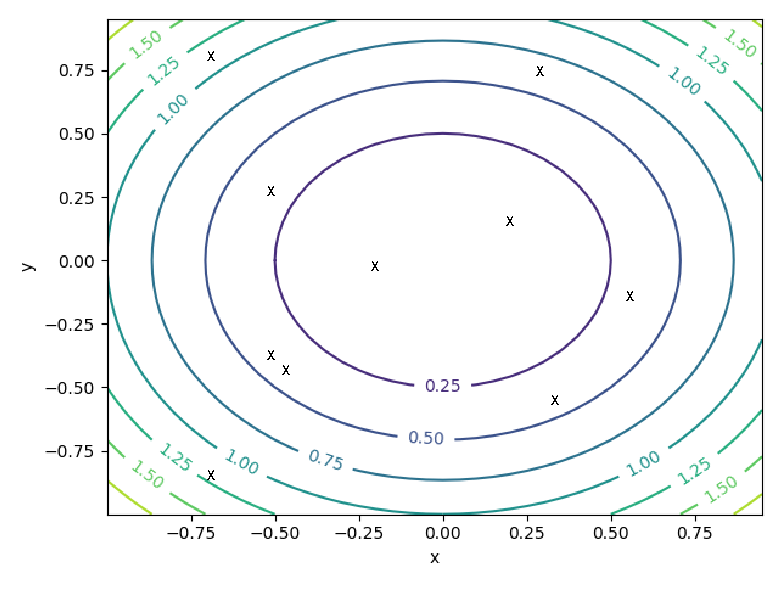
\includegraphics[width=\textwidth]{gfx/Figures/Theory/RandomSearch.pdf}
    \end{subfigure}
    \begin{subfigure}{0.48\textwidth}
        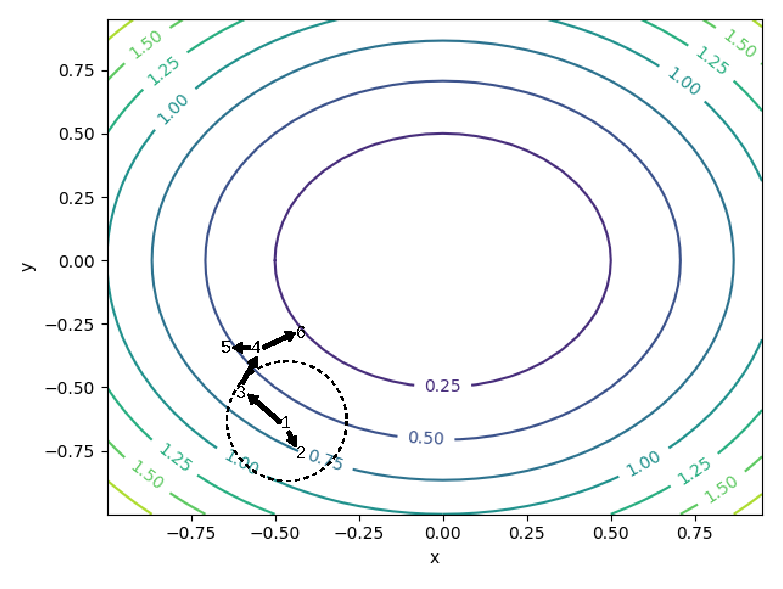
\includegraphics[width=\textwidth]{gfx/Figures/Theory/RandomSearchHypersphere.pdf}
    \end{subfigure}
    \caption{On the left is the first variant with a few randomly selected candidates. On the right are six possible first iterations of the second variant. The hypersphere is only shown for the first candidate.}
    \label{fig:theory:random-search}
\end{figure}

\textbf{Grid Search}: A Grid Search tries to cover with a na\"ive brute-force approach as much of the candidate space as possible.
From each dimension of the candidate space a few values are selected either manual, or more commonly by selecting values from the dimensions allowed range in periodic intervals.
For example, if the x-dimension of the running example should be evaluated in the range $[-1,1]$, depending on the available optimization, potential value selections for this dimension could be $\{-1,0,1\}$ or $\{-0.75,-0.25,0.25,0.75\}$.
With this method the candidate space is discretized and therewith becomes enumerable.\newline
After selecting the value sets for each dimension, the Cartesian product of all sets is calculated.
The elements of this Cartesian product, which are valid candidates because they have a value of each dimension, are the candidates that will be evaluated during the search and for the order of evaluations any arbitrary sequence of the sets elements can be selected.
After either all candidates from the Cartesian product are evaluated or if the optimization budget is spent, the best evaluated candidate is the overall optimization result.
An illustration of a Grid Search over the candidate space of the running example can be seen in figure~\ref{fig:theory:grid-search}.\newline
Therefore, as opposed to Random Searches where by chance only a small portion of the candidate space could be covered, a certain coverage of the space is assured.
Especially in contrast to the second variant of the Random Search, the advantage is that there is no risk of getting stuck in a local optimum.
But im comparison of with the second Random Search variant the main drawback of a Grid Search comes clear, i.e. a Grid Search does not utilize the knowledge gathered from previous evaluations at all, since the evaluation order is completely predefined.
This, even if the Grid Search would evaluate a candidate comparably close to a global optimum, it would completely disregard this chance and not continue the search closely to this candidate to potentially find this global optimum.\newline
Grid Searches are as well as Random Searches classical algorithm choices for Hyperparameter optimization because they are easy to implement and very resource-efficient due to their simplicity such that a high number of candidate evaluation can be performed.
In the context of AutoML, a 2-dimensional Grid Search was utilized in the Weka toolbox~\cite{Witten-Weka} for a simple AutoML approach.
There, a joint candidate space was searched with a set of classifiers for model selection on one dimension and the other dimension is used to select the amount of components of Partial Least Squares filter, which is used as a pre-processor, and can therefore be considered as a simple model configuration.
\begin{figure}[ht!]
    \centering
    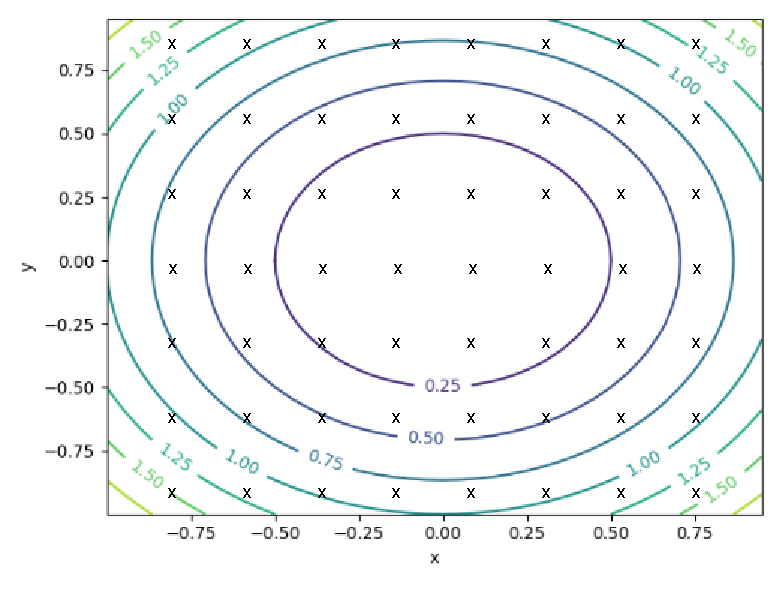
\includegraphics[width=\textwidth]{gfx/Figures/Theory/GridSearch.pdf}
    \caption{Illustration of a Grid Search covering the search space of the running example systematically.}
    \label{fig:theory:grid-search}
\end{figure}

\textbf{(Heuristic) Graph Search}: While a Random Search does it partially leaf to chances which candidates are evaluated, the candidate space will not be adequately covered with a high probability, a Grid Search will have certain coverage guarantees by default.
On the other hand, a Grid Search will not utilize any gathered knowledge about the candidate space while at least the second variant of a Random Search is capable of utilizing knowledge about one prior evaluation.
A Graph Search, usually in combination with a heuristic for search guidance, tries to achieve a trade-off between the advantages of both other presented search algorithms, i.e. having a solid coverage of the candidate space as well as utilizing knowledge gathered during the search.\newline
As the name suggests, for a Graph Search the candidate space is depicted as a graph, but how the space is transformed into a representation consisting out of nodes and edges is very domain and approach specific and several methods exist.
For example, each node could represent a concrete candidate out of the space and can be directly evaluated.
The edges would connect such candidate nodes, if they have a maximum distance to each other, comparable to the hyperspheres the second Random Search variant uses to define neighborhood.
Another method could be to use a tree as a search graph, where only the leaf nodes are concrete candidate nodes, which can be evaluated.
Here, the inner nodes are used to progressively discretize the candidate spaces dimensions in a hierarchical manner by splitting the range into multiple intervals and creating a new child node for each one.
This is continued until the intervals of each dimension either only consist of one element or are small enough such that one value out of it can be selected arbitrarily.
At this point, a leaf node would be the child node because for each dimension a value is selected such that the candidates configuration is complete and could be evaluated.\newline
With a given start node and a method to expand this start node incrementally into a bigger graph, a large amount of search algorithms exists to utilize to search this graph for the best candidate.
They mostly differ in the selection method which unexplored node should be visited next.
The set of nodes, consisting of the unexplored neighbors of already visited and expanded nodes is called a \textit{Search Front} and it is exemplarily illustrated for a search tree in figure~\ref{fig:theory:graph-search-front}.
\begin{figure}[ht!]
    \centering
    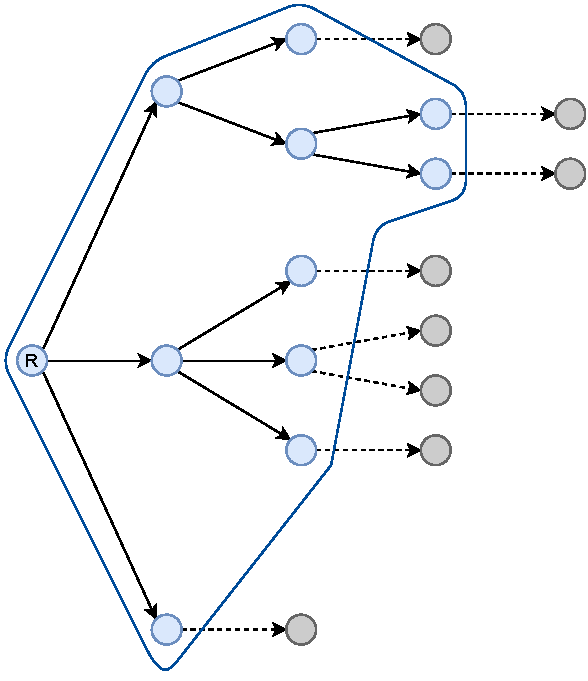
\includegraphics[width=\textwidth]{gfx/Figures/Theory/GraphSearchFront.pdf}
    \caption{After a few iterations of a search algorithm beginning at the root node, a few nodes are already explored and expanded, here illustrated in blue. The expanded child nodes of the searched area(blue) are the search front(grey nodes) and one of them will be explored and expanded in the next search iteration.}
    \label{fig:theory:graph-search-front}
\end{figure}
Some search algorithms select nodes out of the search front  based on the point in time, where they were added to the search front, like for example a Depth-First Search or a Breadth-First Search.
This is a valid approach if the optimization budget is very large and is sufficient to traverse the graph more or less completely.
But in the most use-cases the budget will not even be remotely sufficient for this and the next node out of the search front should be the node, were the best evaluation score or a path to the best evaluation score can be expected.\newline
In the case of the first described method to transform a candidate space into a graph, where each node is a candidate and can be evaluated, this is trivial.
But for the second method, this is more challenging because only leaf nodes can be evaluated and inner nodes not.
To assign a score to a inner node without searching the complete sub-graph below it, an estimation method is utilized, usually called a heuristic.\newline
For example with some available domain knowledge, if certain discretization intervals or selected values are more promising than other, the heuristic can assign higher scores to the corresponding child nodes representing the interval or value.
In the AutoML context this could be done, if for example a certain pipeline component performed outstandingly for previous experiments with this component.
But usually this will not be the case because the relationships between pipeline components to each other and their parameter configuration is too complex and even minor changes can have a big influence to the evaluation score.
Therefore, it is hard to score an incomplete pipeline even with pre-existing domain knowledge.\newline
Without a way to deterministically score a inner node, a probabilistic approach is more promising.
Here, it can be assumed if enough leaf nodes at the end of the sub-graph below the inner node, which shall be scored, are evaluated, it is possible to score the inner node based on these evaluations with a sufficient certainty.
Which path to follow to reach a leaf node in the sub-graph is decided randomly.
To score something based on a a series of random experiments is called a \textit{Monte-Carlo} simulation/experiment and is a common approach to obtain a value, where the exact calculation of the value is either impossible or too complex.
This combination of utilizing a heuristic Graph Search with Monte-Carlo simulations as a heuristic for optimization in the AutoML context was applied to a Best-First Search in the ML-Plan approach~\cite{Mohr-ML-Plan}. 

\subsection{Genetic and Evolutionary Optimization}
\label{sec:theory:optimization:genetic}
Genetic and Evolutionary optimization methods try to transfer the process of the evolution in nature, as described in Charles Darwins \textit{Natural Selection} theory, to computational optimization.
Exactly like an biological evolution model for a species, the optimization process is modelled in consecutive generations and each generation consists out of a high number of individuals.
Ideally, only the individuals which are best adopted to their surroundings should produce offsprings and therefore create a succeeding generation, which is based on this individuals with minor changes.
This is often referred to as \textit{Survival of the fittest}.
Transferred to optimization, this would mean that each individual is a possible solution candidate and therefore a generation is a set of solution candidates.
Starting with a base generation of usually randomly created individuals, a Genetic Algorithm follows the following pattern:
\begin{enumerate}
    \item Evaluate each individual of the current generation.
    \item Select a subset of the current generation that will be used to create the next generation. Normally, this subset is created as a mix of the highest scoring individuals as well as some randomly selected individuals to prevent focussing on local optimums. But other selection approaches were also developed.
    \item Generate the next generation with the selected subset. A pre-defined ratio of individuals will be directly copied into the next generation and the remaining individuals will be modified with evolutionary operators to attempt an enhancement.
\end{enumerate}
This steps are usually repeated until either a certain target score is achieved with one individual, the optimization budget is spent or the scores did not improve over the last $n$ generations.\newline
The aforementioned evolutionary operators work on so called \textit{genetic representations} of candidates, sometimes also called \textit{Genomes} or \textit{Chromosomes}.
In theory nearly every data structure is a suitable for this representation but most often are simple arrays or vectors used, where each cell represents one property of the candidates or alternatively one dimension of the candidate space.
For the running example this would mean an array with length 2, one for the $x$ and one for the $y$ dimension.\newline
Just as in the general principle from biological evolution, these genomes can change by random mutations as well as by recombination, when two individuals produce a new individual.
For a mutation, one individual is selected and one or more cells are changed slightly at random and the other values are kept the same.
If the amount of cells to change is not pre-defined, this is the same idea of randomly selecting a candidate out of hypersphere around another candidate already mentioned for Random Searches.
Thus, if the only applied evolutionary operator is the mutation operator, a Genetic Algorithm would be conceptually comparable to multiple parallel running Random Search instances, but in combination with the recombination operator this Random Search instances can interact with each other and re-organize their current positions to increase the chance of a high candidate space coverage.\newline
A recombination based on two genomes $g_1$ and $g_2$ to produce a new genome $g^*$ is usually performed as a cross-over.
For each cell of $g^*$ the value is taken from either $g_1$ or $g_2$.
Depending on the type of cross-over, there $k \in [1 ... |g^*| - 1]$ cross-over points, which are selected randomly.
Each cross-over point marks an index of $g^*$ at which it will be switched from $g_1$ to $g_2$ or vice versa from which source genome the next value will be taken from.
An example for a two-point cross-over is shown in figure~\ref{fig:theory:crossover}.
\begin{figure}[ht!]
    \centering
    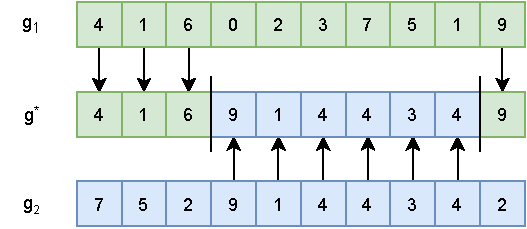
\includegraphics[width=\textwidth]{gfx/Figures/Theory/Crossover.pdf}
    \caption{An example of a two-point cross-over to produce $g^*$ from $g_1$ and $g_2$.}
    \label{fig:theory:crossover}
\end{figure}
With the random factors during selecting the individuals for the generation of the next generation as well as during the application of the evolutionary operators, Genetic and Evolutionary optimization approaches are a stochastic optimization method just as a Random Search or certain Graph Search algorithms and heuristics.
Therefore, the chances of finding a high scoring solution, the coverage of the candidate space as well as the risk of ending in a local optimum are highly dependent on the number of iterations the algorithm performs as well as other configuration parameters like for example the size of each generation.\newline
Additionally to the challenges of handling chances and probabilities emerging from any probabilistic approach, in the context of AutoML there is one more major challenge in applying a Genetic Algorithm for optimization.
A more complicated data structure is needed to represent a pipeline configuration as a single genome because usually they do not have a maximal length and can be composed as a arbitrary graph or tree, which can not represented in an array.
Even if a suitable data structure is found, the mutation and cross-over implementations have to be made very cautious, because representations of pipelines can be very error-prone.
Already small changes to one representation value can lead to an invalid pipeline constructions which cannot be instantiated.\newline
Two state-of-the-art approaches tackling this challenges and applying Genetic Algorithms as optimizers for AutoML problems are \textit{TPOT}~\cite{Olson-Tpot}, using expression trees as a data structure, and \textit{RECIPE}~\cite{Guimar-Recipe}, using grammar-based genetic programming.

\subsection{Bayesian Optimization}
\label{sec:theory:optimization:bayesian}
From all the aforementioned optimization methods, Bayesian optimization utilizes the knowledge from previous candidate evaluations the most.
The goal is to select the most promising candidate for the next evaluation and therefore minimize the overall amount of evaluations until a near-optimal score is reached.
Since each evaluation in the context of AutoML comes with assembling a candidate pipeline and usually performing a cross-validation of the pipeline on the dataset, each evaluation consumes a lot optimization budget.
Therewith, Bayesian Optimization is one of the most used Black Box optimization approaches in recent AutoML research.\newline
The notation of a \textit{most promising} candidate could be interpreted in different ways.
For example, a candidate near the current optimum, which has a high probability of having a comparable or even better score, or a candidate in a completely unevaluated region of the candidate space, where therefore a optimum could lie unnoticed.
But in the case of Bayesian Optimization, this notation of most promising is more sophisticated.\newline
In general, the goal is to create with Bayesian statistics a surrogate function model that replicates the unknown target function as closely as possible.
To model the Bayesian surrogate a common choice is a regression based on a Gaussian Process.
Detailed information about Gaussian Processes can be found for example in~\cite{Rasmussen-Gaussian-Processes}.\newline
This surrogate is based on several evaluations as samples and will become more precise with each new sample, which is usually the next most promising candidate.
For the actual selection of the next most promising candidate sample, a so called \textit{Acquisition Function} is used and the next value will be at an optimum of this acquisition function.
The value of such an acquisition function for a candidate are based on two factors:
\begin{enumerate}
    \item The estimated score of the candidate based on the modelled Bayesian surrogate.
    \item The size of the credible interval of the Bayesian surrogate model at the position of the candidate.
\end{enumerate}
The size of the credible interval is especially important, because if at a point this interval is very broad, the chances are higher that the value of the target function can differ widely from the surrogate at this position.
Of course it can differ in both directions but this can be examined with an additional sample at this position.
Therefore, if the estimated value already indicates an optimum and additionally the credible interval is broad, the value of the target function could be even more optimal at this position and it is the most promising candidate to be drawn as the next sample.
For candidates that were already evaluated, this acquisition score is set to zero because the target score at this position is already known and the surrogate can be certain at this position.
A graphical intuition for the concept of acquisition functions is given in figure~\ref{fig:theory:acquisition-function}, where Bayesian optimization on one dimension of the running example is illustrated.
\begin{figure}[ht!]
    \centering
    \begin{subfigure}{\textwidth}
        \centering
        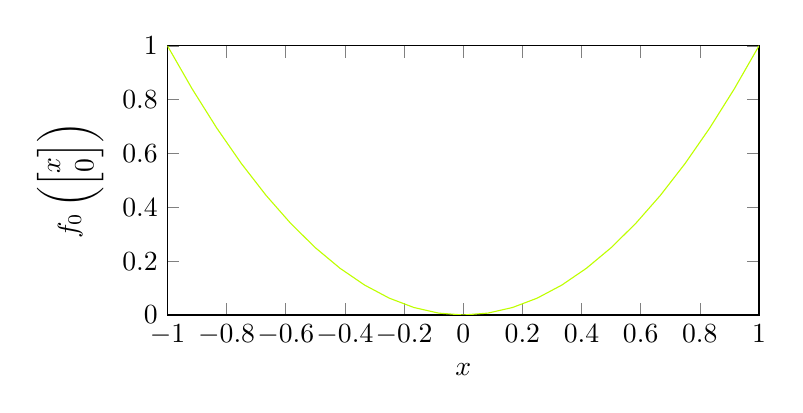
\begin{tikzpicture}
            \begin{axis}[
                xmin=-1, xmax=1,
                ymin=0, ymax=1,
                domain=-1:1,
                xlabel=$x$,
                ylabel=$f_0 \left( \begin{bmatrix}x\\0 \end{bmatrix} \right) $,
                no markers,
                height=5cm,
                width=0.75\textwidth,
            ]
                \addplot[lime]{x^2};
            \end{axis}
        \end{tikzpicture}
        \caption[.]{Slice of the target function $f_0$ at $y=0$.}
    \end{subfigure}
    \begin{subfigure}{\textwidth}
        \centering
        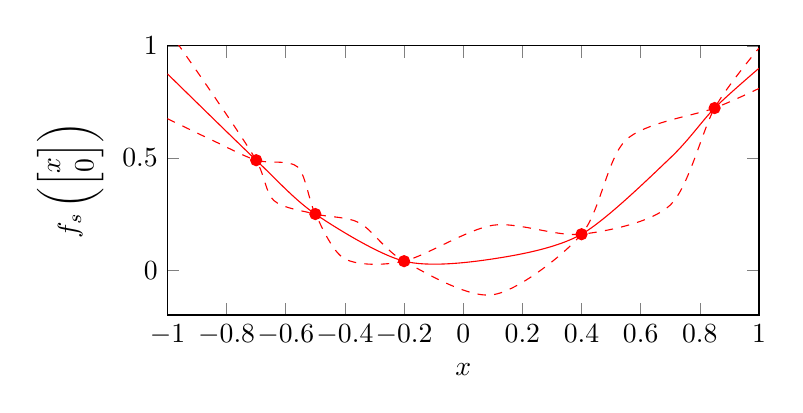
\begin{tikzpicture}
            \begin{axis}[
                xmin=-1, xmax=1,
                ymin=-0.2, ymax=1,
                domain=-1:1,
                xlabel=$x$,
                ylabel=$f_s \left( \begin{bmatrix}x\\0 \end{bmatrix} \right) $,
                height=5cm,
                width=0.75\textwidth,
            ]
                \addplot [only marks,red] coordinates {(-0.7,0.49) (-0.5,0.25) (-0.2,0.04) (0.4,0.16) (0.85,0.7225)};
                \addplot [,
                    smooth,
                    no marks,
                    solid,
                    line join = round,
                    red
                ] coordinates {(-1,0.875) (-0.7,0.49) (-0.5,0.25) (-0.2,0.04) (0.1,0.05) (0.4,0.16) (0.7,0.5) (0.85,0.7225) (1,0.9)};
                \addplot [,
                    smooth,
                    no marks,
                    dashed,
                    line join = round,
                    red
                ] coordinates {(-1,0.675) (-0.85,0.58) (-0.7,0.49) (-0.56,0.46) (-0.5,0.25) (-0.4,0.05) (-0.2,0.04) (0.1,0.2) (0.4,0.16) (0.7,0.29) (0.85,0.7225) (1,0.99)};
                \addplot [,
                    smooth,
                    no marks,
                    dashed,
                    line join = round,
                    red
                ] coordinates {(-1,1.075) (-0.85,0.79) (-0.7,0.49) (-0.64,0.31) (-0.5,0.25) (-0.35,0.21) (-0.2,0.04) (0.1,-0.11) (0.4,0.16) (0.55,0.58) (0.85,0.7225) (1,0.81)};
            \end{axis}
        \end{tikzpicture}
        \caption[.]{
            Estimated surrogate function $f_s$ modelled after 5 samples.
            The evaluated samples are shown as red dots, the surrogate function as a red line and the credible intervals as the two red dashed lines.
            Important note: The values of the surrogate function and the credible intervals are not actually calculated but are only rough estimates to give an intuition of the method.
        }
    \end{subfigure}
    \begin{subfigure}{\textwidth}
        \centering
        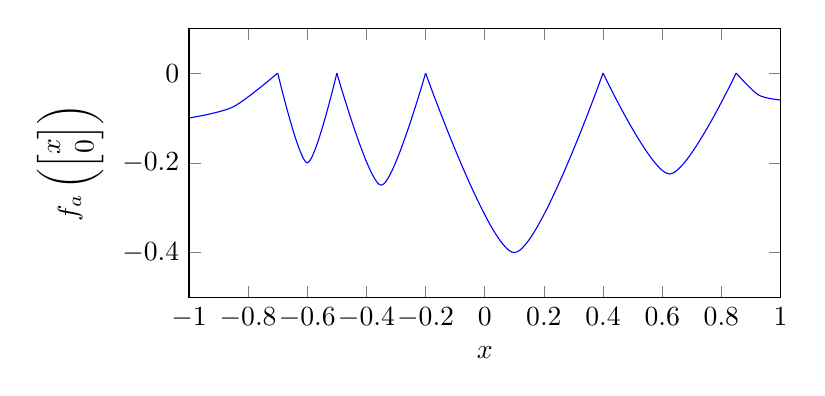
\begin{tikzpicture}
            \begin{axis}[
                xmin=-1, xmax=1,
                ymin=-0.5, ymax=0.1,
                domain=-1:1,
                xlabel=$x$,
                ylabel=$f_a \left( \begin{bmatrix}x\\0 \end{bmatrix} \right) $,
                height=5cm,
                width=0.75\textwidth,
            ]
                \addplot [,
                    smooth,
                    no marks,
                    solid,
                    line join = round,
                    blue
                ] coordinates {(-1,-0.1) (-0.85,-0.075) (-0.7,0)};
                \addplot [,
                    smooth,
                    no marks,
                    solid,
                    line join = round,
                    blue
                ] coordinates {(-0.7,0) (-0.6,-0.2) (-0.5,0)};
                \addplot [,
                    smooth,
                    no marks,
                    solid,
                    line join = round,
                    blue
                ] coordinates {(-0.5,0) (-0.35,-0.25) (-0.2,0)};
                \addplot [,
                    smooth,
                    no marks,
                    solid,
                    line join = round,
                    blue
                ] coordinates {(-0.2,0) (0.1,-0.4) (0.4,0)};
                \addplot [,
                    smooth,
                    no marks,
                    solid,
                    line join = round,
                    blue
                ] coordinates {(0.4,0) (0.625,-0.225) (0.85,0)};
                \addplot [,
                    smooth,
                    no marks,
                    solid,
                    line join = round,
                    blue
                ] coordinates {(0.85,0) (0.925,-0.0485) (1,-0.06)};
            \end{axis}
        \end{tikzpicture}
        \caption[.]{
            Acquisition function $f_a$ based on $f_s$ and its credible intervals after the 5 samples in.
            As in (b), the values are only estimations and not explicitly calculated.
            The minimum of $f_a$ at $x=0.1$ would be the best choice for the sixth sample.
            There the expected value of the surrogate regression is already low and the credible interval is additionally broad.
        }
    \end{subfigure}
    \caption[.]{
        Simple illustration to give an intuition of acquisition functions for the running example of minimizing $f_0 \left( \begin{bmatrix}x\\y \end{bmatrix} \right) = x^2 + y^2$.
        For simplicity will the Bayesian optimization only be used to minimize on the x-dimension and y will be set to 0, but in theory can this approach be extended to any number of dimensions.
        (a) shows a slice of the target function in green.
        (b) shows in red the already evaluated samples, the estimated surrogate function model and the credible intervals.
        (c) shows in blue the acquisition function based on the values in (b).
    }
    \label{fig:theory:acquisition-function}
\end{figure}
An exemplaric algorithm for Bayesian Optimization is given by~\textcite{Frazier-Bayesian-Optimization} with the following pseudo-code in algorithm~\ref{alg:bayesian-optimization}.
\begin{algorithm}[ht!]
    \SetAlgoLined
    Place a Gaussian process prior on $f$\;
    Observe $f$ at $n_0$ points according to an initial space-filling experimental design\;
    Set $n=n_0$\;
    \While{$n \leq N$}{
        Update posterior probability distribution on $f$ using all data\;
        Let $x_n$ be a maximizer of the acquisition function over $x$, where the acquisition function is computed using the current posterior distribution\;
        Observe $y_n = f(x_n)$\;
        Increment $n$\;
    }
    Return a solution: either the point with the largest $f(x)$, or the point with the largest posterior mean\;
    \caption{Basic pseudo-code for Bayesian optimization}
    \label{alg:bayesian-optimization}
\end{algorithm}
The functionality of this pseudo-code as well as some technical terms are explained in the following line by line:
\begin{enumerate}
    \item A probably distribution, for example a Normal distribution is selected as a initial prior distribution $f_0$ to further construct the surrogate function with.
    \item Since this initial $f_0$ is not very meaningful regarding the target function, a few candidates will be evaluated before the actual optimization loop starts.
    This candidates are selected to be a space-filling design, which means to have the best coverage of the candidate space.
    Therewith, the credible intervals between the initially observed points can be kept as small as possible before the acquisition function, which uses this intervals, is used.
    An example for a simple space-filling experiment design is to chose candidates uniformly distributed in the candidate space.
    \item Since this implementation uses the number of observations of $f$ for a given point, i.e. candidate evaluations, as a optimization budget, the variable $n$, which keeps track of the spent budget, is set to $n_0$, because this is the amount of initial evaluations.
    \item Here starts the main optimization loop.
    As long as the optimization budget is not spent and therefore $n \leq N$, further candidates can be selected and evaluated.
    \item Let $d_n$ be all evaluated points from previous iterations or from $n_0$, the surrogate function model of this iteration $f_n$ will be updated based on $d_n$.
    Therefore, a new surrogate function posterior probability distribution is calculated by updating the chosen distribution with the previous posterior distribution $f_{n-1}$ as i new prior, i.e. $f_n := f(x)|f_{n-1}$.
    \item $x_n$ is selected to be the candidate of this iteration for evaluation. It is chosen by searching the acquisition function, which was updated with the data from prior iterations, for an optimum.
    \item Get a evaluation score $y_n$ for the selected candidate of this iteration $x_n$ by observing the $f(x_n)$, thus having one more data point to base to posterior probability distribution on, to construct a more precise surrogate function $f_{n+1}$ in the next iteration.
    \item Increment $n$ because another candidate evaluation was performed and therefore the remaining optimization budget decreased.
    \item The optimization budget is spent and the main optimization loop will terminate.
    \item After the main optimization loop finishes, the algorithm will terminate and return a candidate as the result.
    It will select the best candidate among the evaluated points so far and compare it to the point with the largest posterior mean, i.e. the point where the global optimum, based on the overall constructed surrogate function $f_N$, is assumed.
    If this point is assumed better than the best evaluated candidate it will be returned and the best evaluated candidate otherwise.
\end{enumerate}
A state-of-the-art implementation of Bayesian optimization for algorithm configuration problems is \textit{SMAC}~\cite{Hutter-SMAC}, an abbreviation for Sequential Model-Based Optimization for General Algorithm Configuration.
It is utilized as an optimization approach for a joined model selection and model configuration AutoML optimization space by several approaches, including \textit{Auto-WEKA}~\cite{Thornton-AutoWeka} and \textit{auto-sklearn}~\cite{Feurer-AutoSklearn}.

\subsection{No-Free-Lunch Theorem}
\label{sec:theory:optimization:lunch}
The state-of-the-art AutoML approaches presented with their corresponding black-box optimization method have one thing in common: They all apply a single optimization algorithm to find the best candidate from a optimization space, which is a joined model selection and model configuration space.
While this is a valid approach and will found an optimal or near optimal solution for many AutoML problem instances, it is theoretically impossible that the best solution can be found with a single optimization method for every AutoML problem instance.
This can be deduced from the \textit{No-free-lunch Theorems}, which were proven for optimization problems by~\textcite{Wolpert-No-Free-Lunch-Theorems}.
In these theorems is stated that when an optimization algorithm performs superior for one problem or class of problems, it has to pay for this by performing inferior for other problems.
Of course this is only the case for optimizing with an optimization budget, because the most optimization algorithms can find the best solution if they have an unlimited budget, even if its just by simply evaluating each possible candidate.\newline
For the context of the AutoML setting, the notion of a problem class could for example be transferred to the data, which is given as an input.
Therefore, in this setting with a limited budget of time or resources, one single optimization algorithm may find the best models and configurations for some datasets but cannot achieve this for all datasets.
Thus, the presented AutoML approaches incapable of being the superior approach for all datasets.
With a given dataset $D_1$ a Genetic Algorithm may find the best solution, while a Bayesian optimization method outperforms the same Genetic Algorithm for another dateset $D_2$.\newline
It is additionally possible that the quality of an optimizer does not only depend on the input dataset, i.e. the AutoML problem class, but additionally on the concrete optimization space it operates in and the optimization budget.
This three components could be used to construct a specific problem instance for a dataset problem class.
If this optimization space is modified and thus a new problem instance $p_2$ is created from the original problem instance $p_1$, this can have a huge influence on the optimizer qualities and the optimization method that was the most successful one for $p_1$ could now theoretically be the worst one for $p_2$.\newline
Such a modification of the optimization space can be created if, for instance, the model selection part is already finished and the remaining model configuration induces the optimization space, which is now the problem of optimizing the parameters of a concrete pipeline.
Here, different optimization spaces can be created out of one initial space by pre-selecting a pipeline and different optimizers can differ in quality here as well.
For example, with a given dataset, optimizer $A$ could find good configurations for a pipeline consisting of a Principal Component Analysis followed by a Decision Tree, while optimizer $B$ does this better in the case of a single Support Vector Machine.
The same transformations of the optimization space can of course as well be done by only considering model selection instead and not model configuration.\newline
Since one optimization method will only be the best one for a limited set problem classes, it can be beneficial to use more than one optimization method together for different transformations of the optimization space to extend the set of problem classes, where these combined optimizers can be superior.\newline
In the next section a selection of approaches from related works approaches will be presented, which use such transformations of the optimization space and different optimizers for the transformations, to utilize this extension of problem classes in the AutoML context, where superiority can be achieved.

\section{Related Work}
\label{sec:theory:related}
The first presented approach that uses different optimizers for different transformed AutoML optimization spaces is \textit{ReinBo}~\cite{Sun-ReinBo}.
Here, the overall optimization space, containing model selection and model configuration, is transformed into a solely model selection space at first.
For practicability each pipeline can only consist out of up to three components: One for data pre-processing, one for feature engineering, and one as the machine learning model.
The model selection is performed in three stages, in each of which one of the three component types is selected successively.
It is also possible to not select any component for a pre-processing or feature engineering, which could be represented by a symbol like for example "NA".
A simple example for a small optimization space for such a model selection method would therefore consist out of three sets:
\begin{itemize}
    \item A set $S_p$ with pre-processing algorithms: For example $S_p=\{$Min-Max Scaling, One-Hot Encoding, NA$\}$
    \item A set $S_f$ with feature engineering methods: For example $S_f=\{$ PCA, Variant Threshold Filtering, NA$\}$
    \item A set $S_m$ with machine learning models: For example $S_m=\{$ SVM, Decision Tree$\}$
\end{itemize}
Such a model selection space as in ReinBo can be imagined as a tree, where the root is an empty pipeline that has none of the three component types selected.
This root node has a child node for each $s_p \in S_p$, including the representation symbol "NA" for not selecting any pre-processing component.
Therefore, the child node which represents one $s_p$ means that the pipeline from this sub-tree uses $s_p$ as a pre-processor.
Accordingly, such a child node for a $s_p \in S_p$ has a child node itself for each $s_f \in S_f$ and ultimately each $s_f$ node has a child node as well for each $s_m \in S_m$, which now is a leaf node since the pipeline components are completely constructed.
An illustration of the previous example optimization space can be seen in figure~\ref{fig:theory:reinbo-model-selection}.
\begin{figure}[ht!]
    \centering
    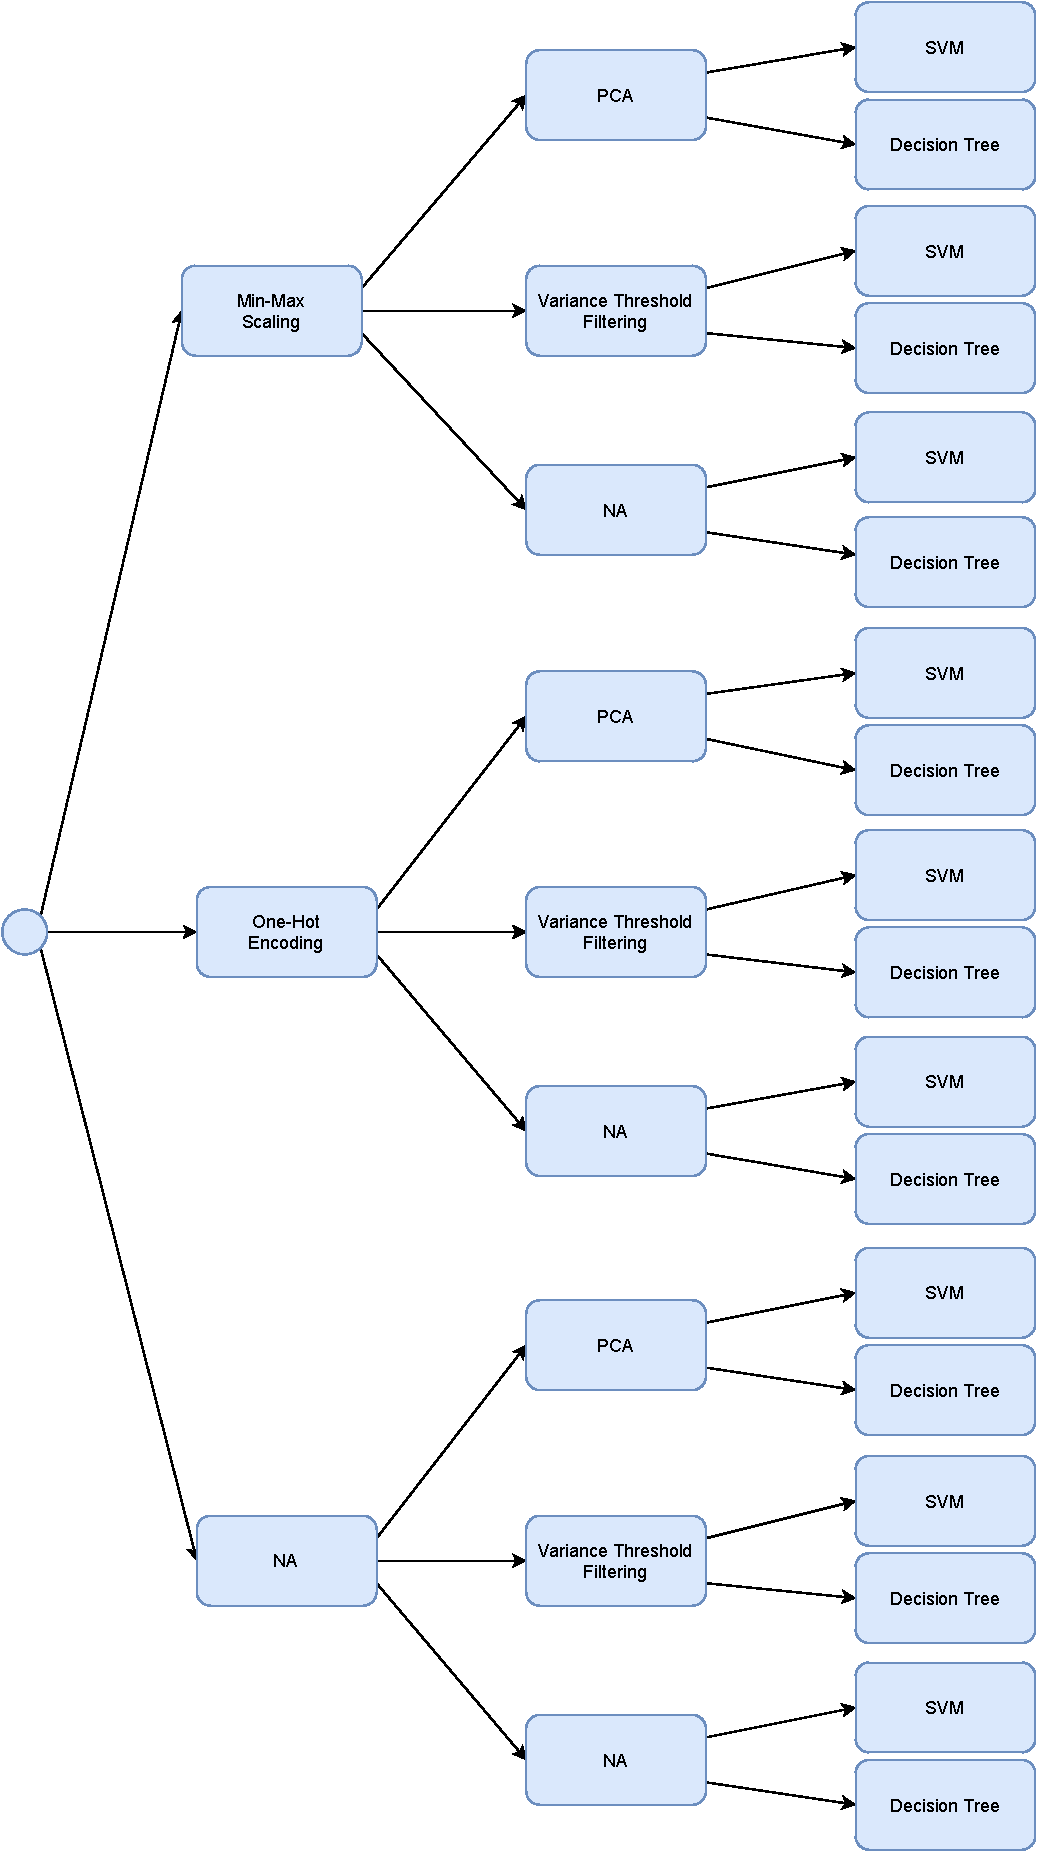
\includegraphics[width=\textwidth]{gfx/Figures/Theory/ReinBoModelSelection.pdf}
    \caption{Simple visualization of the underlying concepts of the three layer ReinBo model selection candidate space.}
    \label{fig:theory:reinbo-model-selection}
\end{figure}
Because of the tree-like structure of this optimization space, a hierarchical Reinforcement Learning approach is trained during the optimization.
With learning about suitable pipeline component choices, it can act as an optimizer for model selection.\newline
After the Reinforcement Learning model has selected up to three pipeline components, the possible parametrization of each component is examined.
From the possible parametrization of each selected component a model configuration space can be induced.
Therewith, based on a completed model selection, the overall optimization space is once more transformed, but now to a space representing possible model configurations for the constructed pipeline.
Each leaf node of the tree structure has such a small model configuration space.\newline
Once the Reinforcement learning model performed the action of selecting a component from the last hierarchical layer and it reaches such a leaf node, Bayesian optimization is conducted in the model configuration space of this leaf.
The evaluation result of the best candidate of this optimization run is given as a reward to the Reinforcement Learning model such that it can update its policy.
Afterwards, in next iteration the Reinforcement Learning model starts once again in the root node and has to select pipeline components based on the policy and this is repeated until the optimization budget ist spent.\newline
Because Bayesian optimization is not very effective for high dimensional spaces, it is a suitable approach to not running a Bayesian optimization on the complete candidate space as an optimization approach.
Instead the model selection is performed by another optimizer and only a small portion of the model configuration space is the input for a Bayesian optimization run, which includes only the hyperparameter of the selected components.
The dimensionality is reduced to a great degree and Bayesian optimization will be more successful.\newline
But this improvements regarding the Bayesian optimization and the inclusion of a Reinforcement Learning model as an additional optimizer, does not extend the set of problem classes where this approach can be superior drastically, because there is still a big amount of problem classes where the Bayesian optimization method itself is not suitable.\newline
\newline
Second, another approach utilizing several optimization phases was publicized by~\textcite{Quemy-Two-Stage-Optimization}.

% !TEX root = ../my-thesis.tex
%
\chapter{AutoML with an Ensemble of Optimizers}
\label{sec:approach}
As outlined in the previous chapter, in theory any optimization approach under a resource budget is limited to a set of problem classes, where it can find a solution that is better than any solution another optimization approach could find for the same problem class, i.e. where the approach is superior.
For an actual use-case, as for instance AutoML, it would be necessary to either have significant domain knowledge or to had conducted a broad empirical evaluation to select the optimizer that have a high chance of performing superior for a newly encountered problem class.
This can be avoided, if during the optimization process a set of optimizers would be evaluated in the context of the presented optimization problem and the most apt one would be applied automatically.\newline
Furthermore, it was argued how a separation of the optimization space into model selection and model configuration spaces by optimization space transformations could be beneficial.
The anticipated advantages are a speed-up at first, because the dimensionality of the input space for an optimizer can be reduced.
Secondly, the best suited optimizer for the model configuration can be selected independently from the constructed pipeline after the model selection.\newline
Although this approach could be generalized to any form of algorithm selection and hyperparameter configuration problem, this thesis focusses on the AutoML use-case and therewith has to address well suited machine learning pipelines as an expected output for a wide variety of datasets as an input.
Thus, the constructed pipelines should be able to be as sophisticated as necessary to suit the complexity of any possible input dataset.
Therewith, the approach has the additional requirement of preventing overly stringent limitations of the pipeline topology such as a fix length or solely linear compositions.\newline
In the following chapter such a method will be presented and applied to the AutoML use-case.
This approach will be explained in the following steps in separate sections:
\begin{enumerate}
    \item A short overview how model selection and configuration spaces can be separated for this approach
    \item The structure of the model selection optimization space and how the optimization will be performed to enable the selection of different optimizers for model configuration out of an embedded optimizer ensemble
    \item The structure of the model configuration optimization space and which benefits can be utilized from using and re-using the different optimizers of the ensemble
\end{enumerate}

\section{Separation of Model Selection and Configuration}
\label{sec:approach:separation}
A usual AutoML optimization search space is a joint space for model selection and model configuration consisting out of a set of components, which can be used to construct a machine learning pipeline, and based on the selected components, a valid configuration has to be created.
Since in the joint optimization space the selected components are not known beforehand, the dimensionality of this space has to be selected for a fix parametrization size.
Hence, the model configuration can only create parameter configurations with a pre-defined size as a constraint and the set of pipeline components for model selection can only contain components whose configuration does not exceed this size.\newline
If the model selection and the model configuration steps are performed sequentially on separated optimization spaces, the dimensionality of the model configuration space can depend on the outcome of the model selection step and have the necessary dimensionality for the constructed pipelines parametrization.\newline
Similar to ReinBo and Mosaic, the model selection space is represented by a tree structure.
After the optimization method reaches a leaf node and has therewith complete and valid pipeline structure, the size of the required configuration becomes clear.
Any leaf node is for this reason the connection point and foundation for a model configuration space and the configuration requirements can be deduced.
Thus, dimensionality and structure of the optimization space for the model configuration can be determined from the configuration requirements of the pipeline represented in this leaf node.

\section{Model Selection with MCTS}
\label{sec:approach:selection}
While the overall goal of the model selection step is to construct a pipeline out of a set of pipeline components, in this approach two additional sub-goals come in addition as supplementary requirements:
\begin{enumerate}
    \item The constructed pipeline should be able to be constructed more flexible and more sophisticated than in ReinBo and Mosaic, i.e. have an unrestricted length and no constraints regarding linearity.
    \item The model selection step should be able to evaluate the different optimization methods and their performance regarding the input dataset or even regarding the model configuration for specific pipeline components in the context in the dataset.
    With such an approach, the the most suitable optimizer can be detected and exploited, which will be the key concept for creating an optimizer ensemble.
\end{enumerate}
In the following, both sub-goals will be addressed.
The next two sub-sections tackle the first sub-goal by modelling the model selection process as a graph search problem as first and describing this search graph in more detail afterwards.
Thereafter, in the third sub-section a formalization of the ensemble concept for multiple optimizers is given in the form of a Multi-Armed Bandit problem.
Finally, in the fourth sub-section it is illustrated how both sub-goals can be achieved during the model selection by performing a MCTS.

\subsection{Model Selection as a Graph Search Problem}
\label{sec:appraoch:selection:search}
A machine learning pipeline can vary heavily in structure and complexity.
For example, simple using a Decision tree as the only component as well as many components in a more sophisticated topology as in figure~\ref{fig:appraoch:complex-pipeline} are valid pipelines and depending on the concrete input dataset, both variants could be the optimal output of the model selection step.
\begin{figure}[ht!]
    \centering
    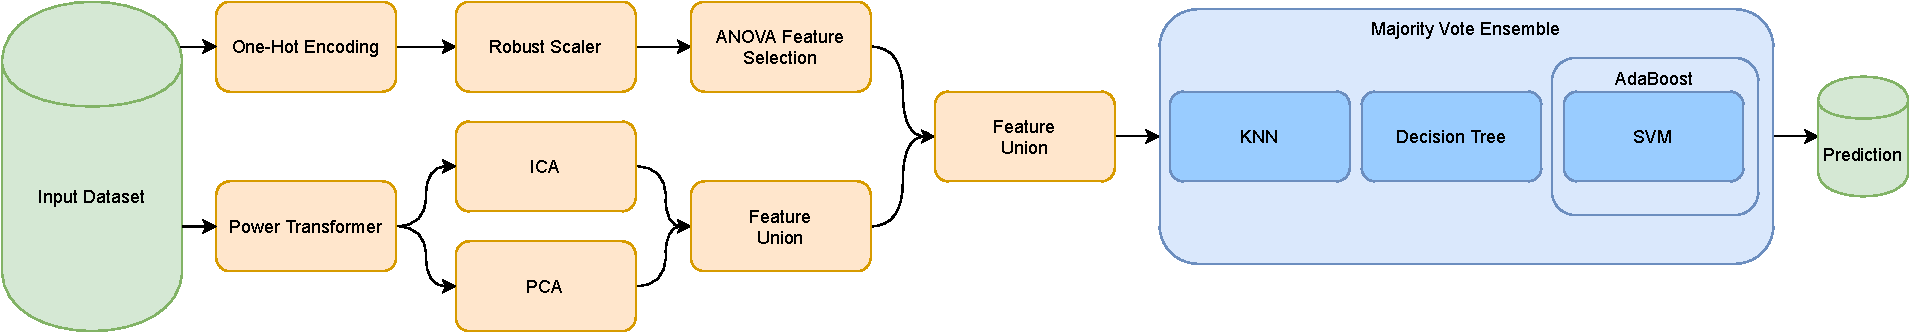
\includegraphics[width=\textwidth]{gfx/Figures/Approach/ComplexPipeline.pdf}
    \caption{An example of a complex machine learning pipeline with a higher length and a non-linear topology. Input dataset and output prediction data are shown in green, pre-processing components in orange and the machine learning components constructing the machine learning model in blue.}
    \label{fig:appraoch:complex-pipeline}
\end{figure}
Since ReinBo and Mosaic solve their model selection tasks by defining a fix pipeline length and creating a model selection tree containing every combinatorial possible combination from a few different component types, these approaches do not allow complex pipelines.\newline
Other approaches, as for example ML-Plan, TPOT or RECIPE utilize hierarchical task network planning (\textit{HTN planning}) combined with a best-first search or expression trees and formal grammars together with genetic programming, to achieve a more unconstrained model selection optimization space.
Because for the ensemble method a MCTS will be required (will be reasoned in~\ref{sec:appraoch:selection:mcts}), which is a heuristic search algorithm like the best-first search as in ML-Plan, this approach will take this HTN planning approach as a foundation to construct the model selection space in the form of a tree.\newline
As the name suggests, HTN planning is based around the notion of tasks and usually one goal task is given as the planning problem input, which would be "\textit{Construct a machine learning pipeline out of a set of components}" in this case.
These tasks can either be primitive tasks or compound task, where the overall goal task usually is a compound task.
Primitive tasks are simple enough be directly achievable without the need for further planning or other calculations.
An example for a primitive task in the AutoML context could be "\textit{Use a Decision tree as a learning model for the pipeline}" as this task can be directly transformed into a pipeline construction command.\newline
Compound tasks on the other hand, are not directly realizable and it is necessary to further decompose the task.
Each compound task can be decomposed into one or most commonly two or more sub-tasks.
Depending on the planning domain, there are decomposition rules where a compound task has one or more possible decompositions.
Such sub-tasks of a compound task can be primitive tasks, again compound tasks or a mixture of both.
If a compound task can be decomposed into solely primitive tasks, this task is directly solvable via the actions of the primitive tasks.
But if the decomposition of the compound task consists out of at least one compound tasks, this child compound task needs to be decomposed recursively as well until it becomes solvable and this solution can be used to solve the original compound task.
The exemplaric AutoML compound tasks "\textit{Construct a machine learning pipeline out of a set of components}" could be decomposed for example into the to smaller compound tasks "\textit{Construct a pre-processing pipeline out of a set of pre-processing components}" and "\textit{Construct a learning model out of a set of machine learning components}".\newline
With this decomposition of compound tasks into different sub-tasks, the hierarchical aspect of HTN planning is added.
A plan as the solution of the planning problem is therefore a task-tree, where each leaf node is a primitive task and each inner node is a compound task.
To create a search tree for a HTN planning problem, solution states, i.e. solved or incomplete task-trees, as well as planning operations to solve an incomplete task-tree, i.e. selecting and applying decomposition rules, need to be represented with nodes and edges.\newline
Here is one common possibility to have each node represent a task-tree and each outgoing edge is a decomposition rule that is applicable to the task-tree of the node.
This edges are therefore connected to nodes, where the represented task-tree is the result of applying this decomposition rule on the previous task-tree.
For a bigger HTN problem an unsolved task-tree will contain a high number of undecomposed compound nodes and therefore an immense amount of decomposition rules would be applicable.
To reduce the maximum degree of the graph and therefore the memory and runtime complexity of most search algorithms, there should not be an outgoing edge for the applicable decomposition rules of each undecomposed compound task.
A simplification is to create an ordering for the undecomposed compound task of the nodes task tree and only create outgoing edges for decomposition rules, which are applicable to the first compound task of this ordering.
The representation of one simple incomplete task tree and two applicable decomposition rules for the first compound task of an ordering is illustrated in figure~\ref{fig:appraoch:htn-planning}.
\begin{figure}[ht!]
    \centering
    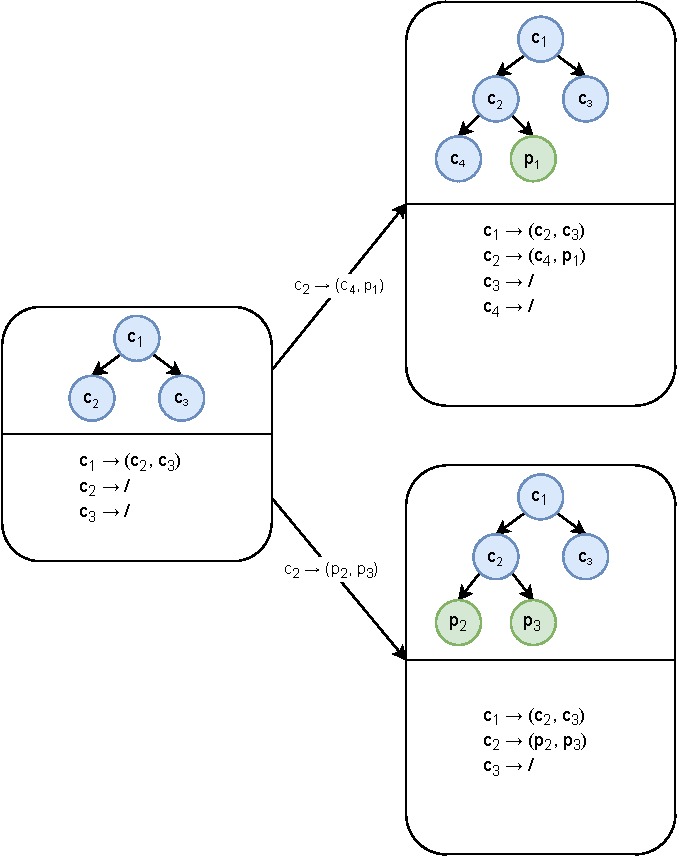
\includegraphics[height=0.5\textheight]{gfx/Figures/Approach/HTN.pdf}
    \caption{An example of a partial HTN planning search tree for a simple planning problem.
    Each node is illustrated with the task-tree for the partially solved plan up to this point in its upper half, where compound task nodes are blue and primitive task nodes are green.
    In the lower half are all involved compound tasks listed in the utilized ordering.
    If any decomposition rule was already applied for a compound task, it is listed here as well.
    The first node on the left has already utilized a decomposition for compound task $c_1$ into $c_2$ and $c_3$.
    In this ordering the first undecomposed compound task is $c_2$ and since two decomposition rules $c_2 \rightarrow (c_4, p_1)$ and $c_2 \rightarrow (p_2, p_3)$ are applicable, the node of this task-tree has two outgoing edges to nodes, where the corresponding decomposition rule was applied to the represented task tree.
    After applying the second decomposition rule, $c_2$ has solely primitive tasks as sub-tasks and can therefore be marked as solved.
    In the case of the first decomposition rule, $c_4$ needs to be decomposed and solved before $c_2$ can would be solved.
    }
    \label{fig:appraoch:htn-planning}
\end{figure}

\subsection{Description of the Search Space Graph}
\label{sec:appraoch:selection:graph}
The examples of HTN tasks in~\ref{sec:appraoch:selection:search} are given as instructions in plain english but this cannot be used in a algorithm and therefore a formalization is necessary.
With a suitable formalization and corresponding data model, the HTN planning domain is adjustable and expandable for the exact use-case and for the case of the AutoML context it is possible to modify possible pipeline topologies and the set of pipeline components that are used for construction.\newline
In a manual pipeline construction it is not possible to create arbitrary pipeline graphs because components often expect a certain type of input that can only be given by certain other components as an output.
Additionally, the selection of some components implies the requirement of selecting certain other components.
For example if an ensemble method was selected as a learning model, the components that are used to be the predictors of the ensemble must be learning model components and cannot be pre-processing models.\newline
To incorporate such constraints into tasks and decomposition rules, ML-Plan utilizes a simple type system in the form of required and provided interfaces.
Each task has one or more type definitions which represents certain properties of the solution to the associated task.
For example, the primitive task of using a Decision Tree as well as the compound task of creating an ensemble learning model out of several other learning models would both offer a solution in the form of a machine learning model.
Both of them could have something like \texttt{Classifier} or \texttt{Learner} as their solution type and therewith as the types of interfaces they provide.\newline
On the other hand, are compound tasks only solvable if they get solutions of certain types as the results of the sub-tasks they are decomposed into.
For example, a Stacking classifier can only be based other classifiers, i.e. solutions with types like \texttt{Classifier}.
Thus, each compound tasks has one or more required interface, which represents this solution types the compound task will be based on.\newline
Decomposition rules are now simple matching rules, i.e. which required interfaces can be satisfied with which provided interface.
Of course it is possible that this interface types need to be identically for simplicity.
A compound task with a required interface of type $a$ can only be decomposed into another task, which has $a$ as one of its provided interface types.
With such a definitions of required and provided interface types for each task, pipeline topology specific constraints like splits into two sub-pipelines and uniting such sub-pipelines, or machine learning specific constraints like for example creating ensembles out of classifiers, are straightforward to incorporate into the planning problem without the need to write a list of decomposition rules.

\subsection{Multiple Optimization Algorithms as a Multi-Armed Bandit Problem}
\label{sec:appraoch:selection:bandit}

\Blindtext

\subsection{Ensemble Interaction with a MCTS}
\label{sec:appraoch:selection:mcts}

\Blindtext

\section{Model Configuration with Multiple Optimizers}
\label{sec:approach:configuration}

\Blindtext

\subsection{Shared Parameter Domain for Selected Models}
\label{sec:appraoch:configuration:parameter}

\Blindtext

\subsection{Warmstarting Versions of Optimization Algorithms}
\label{sec:appraoch:configuration:warmstart}

\Blindtext
% !TEX root = ../my-thesis.tex
%
\chapter{Implementation}
\label{sec:implementation}
The approach of this thesis, described in the previous chapter, is realized as a reference implementation in the \textit{Python} programming language, which can be found here:~\url{https://github.com/Berberer/frankensteins-automl}.
For simplicity and practicability reasons this implementation has some minor restrictions regarding the expected input, but this can be changed or generalized to more inputs with minor modifications.
As for the current implementation state, the optimization budget input is limited to time as the budget and the dataset input has to be in the \textit{ARFF} file format, popularized by \textit{WEKA}~\cite{Witten-Weka}.

This reference implementation serves two different reason:
\begin{itemize}
	\item Help for a better understanding as an alternative and more practical representation of the approach, since it can be easier to read structured code instead of a theoretical and lengthy formal definition.
	\item For the evaluation of this approach and the comparison against other approaches and some baseline values in chapter~\ref{sec:evaluation}, this approach must be provided as an executable program to get results for different experimental settings.
\end{itemize}

The implementation is explained in the following chapter, which is structured in three parts.
At first, the architectural composition of the implementation and the interaction of the included components is explained.
With this overall perspective of the implementation, the codebase will be easier to understand and to navigate.
Since the implementation was not done from scratch, the utilized Python libraries are listed and their functionality explained as a second part to pay respect to their creators as well as elucidate their contribution to the overall functionality.
Finally, the description schema of the AutoML optimization space definition is provided, which is a required input for the implementation, such that a user can understand the included optimization spaces of the implementation and modify them if needed.

\section{Components of the Project and their Interaction}
\label{sec:implementation:components}
The components of the implementation and their architectural composition can be separated into three parts with regard to the subject matter and this separation will be used in the following to outline and explain the implementation.
For the model selection, the search space needs to be constructed from the input optimization space definition.
At first the components for this part of the implementation are explained.
In the second part, the components for evaluating machine learning pipelines and handling the different optimizers are explicated.
All components from this two parts are combined via a MCTS implementation into a overall AutoML program and all components for this are explained in the third part.

\subsection{Model Selection Search Space Management}
\label{sec:implementation:components:search-space}
\Blindtext

\subsection{Pipeline Evaluation and Optimizers for Model Configuration}
\label{sec:implementation:components:optimization}
\Blindtext

\subsection{MCTS and Optimizer Integration}
\label{sec:implementation:components:mcts}
\Blindtext

\section{Utilized Python Libraries}
\label{sec:implementation:libraries}
This reference implementation relies on a few Open-Source Python libraries.
In the following they are listed and their contribution to the functionality of the approach explained in combination with references to their repository and/or creators.
Libraries for development purposes that have not direct influence on the functionality, like for example libraries for unit-testing or code formatting, are omitted from this list but can be seen here:~\url{https://github.com/Berberer/frankensteins-automl/blob/master/requirements.txt}. 
\begin{itemize}
    \item \textit{LIAC-ARFF}\footnote{\url{https://github.com/renatopp/liac-arff}}: A parser for files in the ARFF format to access their data from a Python program.
    \item \textit{NumPy}\footnote{\url{https://github.com/numpy/numpy}}: As a part of the \textit{SciPy} project~\cite{Virtanen-SciPy} for scientific computation, NumPy is an implementation for a wide range of mathematical functions, especially matrix calculation.
    \item \textit{PyPubSub}\footnote{\url{https://github.com/schollii/pypubsub}}: Library for implementing a Publish-Subscribe-Pattern in python for event handling.
    Therewith, if for different events of the AutoML workflow event publishers are added, it is easy to add additional functionality, like for example logging or visualization, as subscriber plug-ins in the form of event listeners, without having to add the plug-ins functionality at every location in the code, where a relevant event occurs.
    \item \textit{scikit-learn}\footnote{\url{https://github.com/scikit-learn/scikit-learn}}: The solved task-trees from the model selection and parametrizations from the model configuration have to be instantiated as a executable machine learning pipeline for evaluation during the optimization and as the final result of the AutoML problem.
    Scikit-learn~\cite{Pedregosa-Scikit-learn} is an established machine learning library with a variety of included components.
    Most of the wanted components for the included components of an AutoML optimization space will be included here and can be referenced simply.
    \item \textit{SMAC v3}\footnote{\url{https://github.com/automl/SMAC3}}: Current version of the official SMAC implementation. It already has new additions to the original approach, as for example warmstarting, included.
\end{itemize}

\section{Exemplaric File Format for defining the AutoML Optimization Space}
\label{sec:implementation:json}
To generate a HTN planning space for the model selection as well as to deduce a model configuration space for a constructed pipeline, a selection AutoML optimization space is required.
This approach implementation has a definition structure for this space in the form of a JSON file in a certain format.\newline
Since it is centered around the HTN planning tasks, which can be translated to pipeline component or pipeline construction steps, this JSON format is an array of components.
Files for the component definitions have the following structure:
\begin{verbatim}
{
    repository: String,
    components: [
        {
            name: String,
            providedInterface: [
                String
            ],
            requiredInterfaces: [
                {
                    name: String,
                    construction_key: String | Number
                }
            ],
            function_pointer ? : Boolean,
            parameter: [
                {
                    name: String,
                    type: String,
                    values ? : [
                        String | Number
                    ]
                    min ? : Number,
                    max ? : Number,
                    default: String | Boolean | Number,
                    construction_key ? : String | Number
                }
            ]
        }
    ]
}
\end{verbatim}

The elements of the definition structure have the following semantic:
\begin{itemize}
	\item \texttt{components}: An array of the components defined in this file. They have each the following structure:
		\begin{itemize}[label=\textbullet]
			\item \texttt{name}: This value is used to resolve the corresponding Python class/function and has therefore to include the Python module path as well as the actual name, like for example "\texttt{sklearn.naive\_bayes.GaussianNB}".
			\item \texttt{providedInterfaces}: This array of string contains unique identifiers for each interface this component provides. With this provided interface and possibly more other provided interfaces, a compound task can be decomposed. 
            \item \texttt{requiredInterfaces}: If this component is represented as a compound task and needs to be decomposed and solved to be instantiable, in this array are definitions for the required interfaces of the decomposition. Each has the following structure:
            \begin{itemize}[label=\textbullet]
                \item \texttt{name}: A unique identifier of a required interface to match valid components against for decomposition.
                \item \texttt{construction\_key}: Since the resolved Python class constructor will be called to instantiate the current component that has this required interfaces, the parameter type signature of the constructor has to be met when calling.
                    Since it will require the resulting component of the solved task of the provided interface matched for this required interface, the resulting component has to be placed an the correct position of the constructor call regarding to the type signature.
                    The construction key can either be a integer to represent the position in the parameter list or a string in the case of a keyword parameter. 
            \end{itemize}
            \item \texttt{function\_pointer}: If this property exists and is set to true, the resolved Python function or constructor will not be actually called and the result returned after resolving the path.
                Instead, a pointer to the resolved function itself will be returned, for the case that another component requires a function as a parameter.
            \item \texttt{parameter}: Most components will require a parametrization if they are added to a pipeline. To deduce the model configuration space for a pipeline, here is a array with with a definition for each parameter the component requires with this structure:
            \begin{itemize}[label=\textbullet]
                \item \texttt{name}: An identifier for this parameter to be distinguishable from other parameters of this component. Hence, it has to be unique in this concrete parameter array.
                \item \texttt{type}: The type of the parameter as a string. Valid values are "int" for integer numbers, "double" for numbers with potential decimal places, "cat" for categorical values(i.e. one out of a pre-defined set of values) and "bool" for a boolean value.
                \item \texttt{values}: If the parameter has the type "cat" this is an array of strings or numbers with the allowed categorical values. If the parameter has another type, this field can be omitted.
                \item \texttt{min} and \texttt{max}: For numerical parameters, i.e. parameters with type "int" or "double" a parameter range for valid values is defined with a minimum and a maximum. For another types, this two fields can be omitted.
                \item \texttt{default}: If the implementation of the represented component has a suitable default value for this parameter, it is defined here as a string, number, or boolean, depending on the parameter type.
                \item \texttt{construction\_key}: Same functionality as the construction key of a required interface.
                    If the component is instantiated, here is defined at which position or with which keyword parameter the parameter value will be passed to the resolved class constructor of this component.
                    Though, for parameters can this property be omitted.
                    In this case it is assumed that the parameter is a keyword parameter and the \texttt{name} property will be used as the keyword.
            \end{itemize}
        \end{itemize}
\end{itemize}
A complete and application-oriented example of an AutoML problem definition in this schema can be found in appendix~\ref{sec:appendix:htn-space}, but for presentation is here the the definition for a scikit-learn feature selection component named SelectPercentile, which can be included in the pre-processing part of a pipeline:
\begin{verbatim}
{
    "name": "sklearn.feature_selection.SelectPercentile",
    "providedInterface": [
        "sklearn.feature_selection.SelectPercentile",
        "FeatureSelection",
        "AbstractPreprocessor",
        "BasicPreprocessor"
    ],
    "requiredInterface": [
        {
            "name": "sklearn.feature_selection.f_classif",
            "construction_key": 0
        }
    ],
    "parameter": [
        {
            "name": "percentile",
            "type": "int",
            "default": 50,
            "min": 1,
            "max": 100,
            "construction_key": "percentile"
        }
    ]
}
\end{verbatim}

% !TEX root = ../my-thesis.tex
%
\chapter{Empirical Analysis and Evaluation}
\label{sec:evaluation}
After devising this approach for optimizer ensembles and implementing it as a reference implementation, it is essential to evaluate and asses this approach.
This assessment is the goal of this chapter and the final step of this thesis before summing up and considering the outcomes of it.\newline
To have a clear guided structure for this assessment, it is based on the research questions presented in~\ref{sec:intro:goal}, which is elucidated here in more detail at first with a focus on which data is required to answer them.
Afterwards, this chapter answers the research questions with a series of Empirical evaluations in the form of experiments.\newline
Therefore, the setup and configuration of the experiments is given as a starting point to subsequently analyze the results of the experiments and to deduce the answers to the research questions from them.

\section{Research Questions in Detail}
The first research question was about the feasibility about the approach, i.e. is it a viable idea to optimize an AutoML problem solution with an optimizer ensemble.
This will be answered in two steps.\newline
At first, are the solution scores of this approach similar or better than the scores of other state-of-the-art approaches for several different datasets?
If they are not at all or not for a high number of datasets, this approach is not a competitor to the state-of-the-art approaches.
In this case, there would be no progress in this scientific field and no motivation to utilize this approach.\newline
Secondly, if there is an improvement in some scores, which component of the approach, the MCTS model selection and the warmstarted optimizer ensemble, has which influence on the improvements.
To assess this influences, three versions of this approach are evaluated, where two of them have slight modifications:
\begin{enumerate}
    \item To evaluate the influence of a Model Selection via a MCTS, the approach does not utilize a optimizer ensemble in this version.
    Every optimizer node represents the same optimizer, which will be SMAC for this evaluation.
    \item To evaluate the influence of the ensembled optimizers, the approach does not utilize a MCTS selection.
    The node selection on each level down the paths to the different optimizer nodes, will be random in each search iteration.
    Therefore, it is basically a repeated random search.
    \item Both components are included in the last version and the full approach is evaluated as described in the two previous chapter. 
\end{enumerate}
By comparing the scores of the tree variants for different datasets and different timeouts, data about the scores with and without one component can be gathered, which can be used to analyze the influence.

As the second research question, the focus is on the utilization of the different optimizers.
During each run of this approach, not for the variants with the modifications, it will be counted how many times each optimizer was selected by the MCTS and therewith started.
Since the MCTS tries to find the best suited optimizer and to exploit it, this selection frequency is an indicator for the suitability of this optimizer to the input dataset.\newline
The frequencies will be aggregated together with the AutoML time budget and the input dataset.
Thus, it is possible to check if one or more optimizers were preferably selected in general or just an AutoML problem setting with a certain time budget or a input dataset with certain properties.
Alternatively, there could be no significant difference and each optimizer was selected comparably often.

\section{Experiment Setup}
\label{sec:evaluation:setup}

\Blindtext

\section{Results of the Experiments}
\label{sec:evaluation:results}

\Blindtext

\section{Analysis of the Experiment Outcomes}
\label{sec:evaluation:analysis}

\Blindtext

% !TEX root = ../my-thesis.tex
%
\chapter{Conclusion}
\label{sec:conclusion}
In this final chapter after previously answering the concrete research questions of the thesis, the prior descriptions and findings regarding the optimizer ensemble AutoML approach are summarized and concluded with an outlook of possible future works.

\section{Summary and Findings}
\label{sec:conclusion:summary}
This thesis was based on the statements of the No-Free-Lunch theorems for optimization, which had proven that under given constraints no optimization algorithm can be superior for all problems.
To approach this problem, the model selection of an AutoML setting combined with choosing an optimizer that should perform a model configuration for the selected pipeline model was seen as a hierarchical Multi-Armed Bandit problem.
Hence, it was tackled with an MCTS, which searches a model selection graph that is realized as an HTN planning graph with embedded optimizers.
This optimizers are combined as an ensemble to utilize each others gathered information about evaluated candidates and perform successive warmstarting for each optimization run.

This novelle AutoML idea was realized as a first simple reference implementation, which afterwards was used in a series of experiments to examine the feasibility of the approach and to gather additional knowledge about the functionality of the components.

In its current reference implementation the approach of this thesis was not able to surpass the currently best state-of-the-art approaches auto-sklearn and TPOT for the examined datasets.
However, it was able to show competitive results for some of the datasets which could indicate the potential to close the current gap between the tools or even surpass them.

\section{Open Questions and Future Work}
Besides the mentioned further development regarding general implementation maturity and optimization, some other factors, which could lead to better results, were not covered by this thesis and are good starting points for future work.
To conclude this chapter, they are listed in the following, grouped into different categories:
\begin{itemize}
    \item \textbf{Configuration}: The evaluation was solely done with one configuration of this approach.
    Although the utilized configuration showed the best results in some tests prior to the experiments, there may exist even better configuration, for example regarding the amount of Monte-Carlo simulations or the time budget of each single optimization run.
    A thorough study of a variety of possible configurations in the context of different AutoML timeouts and more datasets than the evaluated ten, can be a first next step to identify better configurations.\newline
    Additionally, the configuration of this approach remained static during the entire MCTS search.
    Modifying the configuration values during the search, could improve the balance between exploration and exploitation.
    For example, the amount of Monte-Carlo simulation could start with a high value and will be reduced during the run, such that a higher exploration coverage of the search space is reached in the beginning.
    Or alternatively the optimization time budget could start with a low value and be improved later in the search, once the probability of exploiting more suitable optimizers is higher after a certain degree of exploration.
    The adjustment of time budgets, could utilize one of the time allocation policies of~\textcite{Quemy-Two-Stage-Optimization}, which were presented in~\ref{sec:theory:related}.
    \item \textbf{Model Selection Search}: During the evaluation of different configurations, it could also prove worthwhile to evaluate different search algorithms instead of an MCTS.
    Since the variant of this approach that used a random search instead of MCTS was not significantly worse, other search algorithms should also be considered and tested.\newline
    Although MCTS is usually associated with UCT as a policy, there are also other published MCTS policies for scoring nodes and selecting them accordingly.
    A survey of a broad selection of such policies was for example done by~\textcite{Browne-Policies}.
    Besides completely different search algorithms, a study of different MCTS variations and policies could also be a valid starting point for future research.
    \item \textbf{Optimizer Ensemble Model Configuration}: In the case of the evaluated datasets, MCTS rarely exploited a random search or discretization search for optimization in comparison to the other optimizers.
    If this is also the case during a broader study of more datasets, the subset of optimizers that are selected for the ensemble, could be reduced to the remaining three optimizers, or alternatively the two optimizers could be replaced by other optimizers, which were not integrated and evaluated yet.\newline
    Besides the selection of optimizers for the ensembles, the interaction within the ensembles is also a starting point for future research.
    It has to be evaluated if every optimizer really profits from warmstarting or if this leads for example to an over-searching of local optima.\newline
    Similar to adjusting the configuration dynamically during the run, it could also be a variation to enable or disable warmstarting for different time periods of the overall search or for different parts of the search graph.
    In the same manner, early stopping for all or for some optimizers could be added as a functionality and then dynamically be enabled and disabled during the run, if there is a chance for a better budget allocation towards more promising optimizers.\newline
    Additionally, the possibilities for creating the model configuration optimization spaces can be extended to a degree of the expressiveness of auto-sklearns space modelling features.
    Constraints across multiple parameters as for example, "\textit{If value $a$ is selected for parameter $p_1$, value $b$ is no longer an allowed value for parameter $p_2$}" could prevent this approach from evaluating unsuitable or even invalid pipeline parametrization candidates.\newline
    As part of this thesis it was only evaluated if the dataset properties had any correlations to the optimizer utilization, but the same could be done in regard to the components and the topology of the pipeline.
    For example, if one optimization algorithm would be utilized more often for shorter pipelines or alternatively for example, if the learning algorithm is a decision tree, an optmizer selection policy could integrate such correlations.
    \item \textbf{Problem Settings}: In theory, the approach of this thesis has no limitations regarding the desired functionality of the algorithm selection and hyperparameter optimization outcome.
    This thesis focusses on AutoML as one specific outcome, but with minor modifications regarding problem description input and internal candidate evaluation, it can construct models for other combined algorithm selection and configuration domains as well.\newline
    Once the above mentioned improvements were made and this minor modifications for allowing other domains as well, an interesting follow-up research question is to evaluate how the optimizer ensemble approach performs in other domains besides AutoML.
\end{itemize}


% --------------------------
% Back matter
% --------------------------
\appendix\cleardoublepage
% !TEX root = ../my-thesis.tex
%
\chapter{Appendix}
\label{sec:appendix}

\section{Example AutoML Optimization Space Definition}
\label{sec:appendix:htn-space}
This is an adaptation of the model selection and model configuration space of \textit{auto-sklearn}~\cite{Feurer-AutoSklearn} for the approach of this thesis.
It is modelled in the JSON format described in~\ref{sec:implementation:json} for modelling AutoML HTN planning spaces.\newline
Nevertheless, this modelling method is not capable of an exact one-to-one adaptation of the auto-sklearn space because their modelling given as Python code which is as a programming language more expressive than a data interchange language as JSON.
With this modelling in Python, it is possible to create constraints and relationships between parameters of a component.
For example something like if parameter $p_1$ has value $x$, $p_2$ cannot have value $y$, or $p_4$ will only be part of the model configuration if $p_3$ has value $z$.
Additionally, it is possible to include logical processing steps for the selected values after the model configuration in the Python code, for example to change a configured value depending on properties of the actual input dataset.\newline
Improving the modelling capacities of this JSON format can be a starting point for further research.
However, it will not be possible to make it as expressive as the model configuration space definitions in a turing-complete programming language as Python.

In this case it was required for simulating the auto-sklearn search space to have a classifier component and an optional data pre-processor as well as an optional feature pre-procesor.
This concrete search space is split into four parts:
\begin{itemize}
    \item Pipeline Topologies
    \item Data Pre-Processing
    \item Feature Pre-Processing
    \item Classifier
\end{itemize}

\subsection{Pipeline Topologies}
\begin{Verbatim}[fontsize=\scriptsize]
{
  "components": [
        {
            "name": "frankensteins_automl.machine_learning.pipeline.pipeline_constructor.build_topology",
            "providedInterface": ["MLPipeline"],
            "requiredInterface": [
                {
                    "name": "Topology",
                    "construction_key": 0
                }
            ],
            "parameter": []
        },
        {
            "name": "frankensteins_automl.machine_learning.pipeline.pipeline_constructor.topology_union",
            "providedInterface": ["Topology"],
            "requiredInterface": [
                {
                    "name": "PreProcessingTopology",
                    "construction_key": 0
                },
                {
                    "name": "AbstractClassifier",
                    "construction_key": 1
                }
            ],
            "parameter": []
        },
        {
            "name": "frankensteins_automl.machine_learning.pipeline.pipeline_constructor.topology_union",
            "providedInterface": ["Topology"],
            "requiredInterface": [
                {
                    "name": "AbstractClassifier",
                    "construction_key": 0
                }
            ],
            "parameter": []
        },
        {
            "name": "frankensteins_automl.machine_learning.pipeline.pipeline_constructor.topology_union",
            "providedInterface": ["PreProcessingTopology"],
            "requiredInterface": [
                {
                    "name": "AbstractDataPreProcessor",
                    "construction_key": 0
                },
                {
                    "name": "AbstractFeaturePreProcessor",
                    "construction_key": 1
                }
            ],
            "parameter": []
        },
        {
            "name": "frankensteins_automl.machine_learning.pipeline.pipeline_constructor.topology_union",
            "providedInterface": ["PreProcessingTopology"],
            "requiredInterface": [
                {
                    "name": "AbstractDataPreProcessor",
                    "construction_key": 0
                }
            ],
            "parameter": []
        },
        {
            "name": "frankensteins_automl.machine_learning.pipeline.pipeline_constructor.topology_union",
            "providedInterface": ["PreProcessingTopology"],
            "requiredInterface": [
                {
                    "name": "AbstractFeaturePreProcessor",
                    "construction_key": 0
                }
            ],
            "parameter": []
        }
    ]
}
\end{Verbatim}

\subsection{Data Pre-Processing}
\begin{Verbatim}[fontsize=\scriptsize]
{
    "components": [
        {
            "name": "sklearn.preprocessing.OneHotEncoder",
            "providedInterface": ["AbstractDataPreProcessor"],
            "requiredInterface": [],
            "parameter": []
        },
        {
            "name": "sklearn.feature_selection.VarianceThreshold",
            "providedInterface": ["AbstractDataPreProcessor"],
            "requiredInterface": [],
            "parameter": []
        },
        {
            "name": "sklearn.impute.SimpleImputer",
            "providedInterface": ["AbstractDataPreProcessor"],
            "requiredInterface": [],
            "parameter": [
                {
                    "name": "strategy",
                    "type": "cat",
                    "default": "mean",
                    "values": ["mean", "median", "most_frequent", "constant"]
                }
            ]
        },
        {
            "name": "frankensteins_automl.machine_learning.pipeline.pipeline_constructor.topology_union",
            "providedInterface": ["AbstractDataPreProcessor"],
            "requiredInterface": [
                {
                    "name": "DataRescaler",
                    "construction_key": 0
                }
            ],
            "parameter": []
        },
        {
            "name": "sklearn.preprocessing.StandardScaler",
            "providedInterface": ["DataRescaler"],
            "requiredInterface": [],
            "parameter": []
        },
        {
            "name": "sklearn.preprocessing.MinMaxScaler",
            "providedInterface": ["DataRescaler"],
            "requiredInterface": [],
            "parameter": []
        },
        {
            "name": "sklearn.preprocessing.RobustScaler",
            "providedInterface": ["DataRescaler"],
            "requiredInterface": [],
            "parameter": []
        },
        {
            "name": "sklearn.preprocessing.Normalizer",
            "providedInterface": ["DataRescaler"],
            "requiredInterface": [],
            "parameter": []
        },
        {
            "name": "sklearn.preprocessing.QuantileTransformer",
            "providedInterface": ["DataRescaler"],
            "requiredInterface": [],
            "parameter": [
                {
                    "name": "n_quantiles",
                    "type": "int",
                    "default": 1000,
                    "min": 10,
                    "max": 2000
                },
                {
                    "name": "output_distribution",
                    "type": "cat",
                    "default": "uniform",
                    "values": ["uniform", "normal"]
                }
            ]
        }
    ]
}
\end{Verbatim}

\subsection{Feature Pre-Processing}
\begin{Verbatim}[fontsize=\scriptsize]
{
    "components": [
        {
            "name": "frankensteins_automl.machine_learning.pipeline.pipeline_constructor.preprocessor_union",
            "providedInterface": ["AbstractFeaturePreProcessor"],
            "requiredInterface": [
                {
                    "name": "SingleAbstractFeaturePreProcessor",
                    "construction_key": 0
                },
                {
                    "name": "SingleAbstractFeaturePreProcessor",
                    "construction_key": 1
                }
            ],
            "parameter": []
        },
        {
            "name": "frankensteins_automl.machine_learning.pipeline.pipeline_constructor.topology_union",
            "providedInterface": ["AbstractFeaturePreProcessor", "SingleAbstractFeaturePreProcessor"],
            "requiredInterface": [
                {
                    "name": "DecompositionPreProcessor",
                    "construction_key": 0
                }
            ],
            "parameter": []
        },
        {
            "name": "frankensteins_automl.machine_learning.pipeline.pipeline_constructor.topology_union",
            "providedInterface": ["AbstractFeaturePreProcessor", "SingleAbstractFeaturePreProcessor"],
            "requiredInterface": [
                {
                    "name": "FeatureSelectionPreProcessor",
                    "construction_key": 0
                }
            ],
            "parameter": []
        },
        {
            "name": "frankensteins_automl.machine_learning.pipeline.pipeline_constructor.topology_union",
            "providedInterface": ["AbstractFeaturePreProcessor", "SingleAbstractFeaturePreProcessor"],
            "requiredInterface": [
                {
                    "name": "KernelApproximationPreProcessor",
                    "construction_key": 0
                }
            ],
            "parameter": []
        },
        {
            "name": "frankensteins_automl.machine_learning.pipeline.pipeline_constructor.topology_union",
            "providedInterface": ["AbstractFeaturePreProcessor", "SingleAbstractFeaturePreProcessor"],
            "requiredInterface": [
                {
                    "name": "MiscPreProcessor",
                    "construction_key": 0
                }
            ],
            "parameter": []
        },
        {
            "name": "sklearn.decomposition.TruncatedSVD",
            "providedInterface": ["DecompositionPreProcessor"],
            "requiredInterface": [],
            "parameter": [
                {
                    "name": "n_components",
                    "type": "int",
                    "default": 100,
                    "min": 2,
                    "max": 256
                }
            ]
        },
        {
            "name": "sklearn.decomposition.FastICA",
            "providedInterface": ["DecompositionPreProcessor"],
            "requiredInterface": [],
            "parameter": [
                {
                    "name": "n_components",
                    "type": "int",
                    "default": 100,
                    "min": 10,
                    "max": 2000
                },
                {
                    "name": "algorithm",
                    "type": "cat",
                    "default": "parallel",
                    "values": ["parallel", "deflation"]
                },
                {
                    "name": "whiten",
                    "type": "bool",
                    "default": false
                },
                {
                    "name": "fun",
                    "type": "cat",
                    "default": "logcosh",
                    "values": ["logcosh", "exp", "cube"]
                }
            ]
        },
        {
            "name": "sklearn.decomposition.PCA",
            "providedInterface": ["DecompositionPreProcessor"],
            "requiredInterface": [],
            "parameter": [
                {
                    "name": "n_components",
                    "type": "double",
                    "default": 0.9999,
                    "min": 0.5,
                    "max": 0.9999
                },
                {
                    "name": "whiten",
                    "type": "bool",
                    "default": false
                }
            ]
        },
        {
            "name": "sklearn.decomposition.KernelPCA",
            "providedInterface": ["DecompositionPreProcessor"],
            "requiredInterface": [],
            "parameter": [
                {
                    "name": "n_components",
                    "type": "int",
                    "default": 100,
                    "min": 10,
                    "max": 2000
                },
                {
                    "name": "kernel",
                    "type": "cat",
                    "default": "rbf",
                    "values": ["poly", "rbf", "sigmoid", "cosine"]
                },
                {
                    "name": "gamma",
                    "type": "double",
                    "default": 1.0,
                    "min": 3.0517578125e-05,
                    "max": 8.0
                },
                {
                    "name": "degree",
                    "type": "int",
                    "default": 3,
                    "min": 2,
                    "max": 5
                },
                {
                    "name": "coef0",
                    "type": "double",
                    "default": 0,
                    "min": -1,
                    "max": 1
                }
            ]
        },
        {
            "name": "sklearn.feature_selection.SelectFromModel",
            "providedInterface": ["FeatureSelectionPreProcessor"],
            "requiredInterface": [
                {
                    "name": "SelectFromModelEstimator",
                    "construction_key": "estimator"
                }
            ],
            "parameter": []
        },
        {
            "name": "sklearn.feature_selection.GenericUnivariateSelect",
            "providedInterface": ["FeatureSelectionPreProcessor"],
            "requiredInterface": [
                {
                    "name": "FeatureSelectionScoreFunction",
                    "construction_key": "score_func"
                }
            ],
            "parameter": [
                {
                    "name": "mode",
                    "type": "cat",
                    "default": "fpr",
                    "values": ["fpr", "fdr", "fwe"]
                },
                {
                    "name": "param",
                    "type": "double",
                    "default": 0.1,
                    "min": 0.01,
                    "max": 0.5
                }
            ]
        },
        {
            "name": "sklearn.feature_selection.SelectPercentile",
            "providedInterface": ["FeatureSelectionPreProcessor"],
            "requiredInterface": [
                {
                    "name": "FeatureSelectionScoreFunction",
                    "construction_key": "score_func"
                }
            ],
            "parameter": [
                {
                    "name": "percentile",
                    "type": "int",
                    "default": 50,
                    "min": 1,
                    "max": 99
                }
            ]
        },
        {
            "name": "sklearn.feature_selection.chi2",
            "providedInterface": ["FeatureSelectionScoreFunction"],
            "requiredInterface": [],
            "function_pointer": true,
            "parameter": []
        },
        {
            "name": "sklearn.feature_selection.f_classif",
            "providedInterface": ["FeatureSelectionScoreFunction"],
            "requiredInterface": [],
            "function_pointer": true,
            "parameter": []
        },
        {
            "name": "sklearn.feature_selection.mutual_info_classif",
            "providedInterface": ["FeatureSelectionScoreFunction"],
            "requiredInterface": [],
            "function_pointer": true,
            "parameter": []
        },
        {
            "name": "sklearn.kernel_approximation.RBFSampler",
            "providedInterface": ["KernelApproximationPreProcessor"],
            "requiredInterface": [],
            "parameter": [
                {
                    "name": "gamma",
                    "type": "double",
                    "default": 1.0,
                    "min": 3.0517578125e-05,
                    "max": 8.0
                },
                {
                    "name": "n_components",
                    "type": "int",
                    "default": 100,
                    "min": 50,
                    "max": 10000
                }
            ]
        },
        {
            "name": "sklearn.kernel_approximation.Nystroem",
            "providedInterface": ["KernelApproximationPreProcessor"],
            "requiredInterface": [],
            "parameter": [
                {
                    "name": "gamma",
                    "type": "double",
                    "default": 0.1,
                    "min": 3.0517578125e-05,
                    "max": 8.0
                },
                {
                    "name": "n_components",
                    "type": "int",
                    "default": 100,
                    "min": 50,
                    "max": 10000
                },
                {
                    "name": "kernel",
                    "type": "cat",
                    "default": "rbf",
                    "values": ["poly", "rbf", "sigmoid", "cosine", "chi2"]
                },
                {
                    "name": "degree",
                    "type": "int",
                    "default": 3,
                    "min": 2,
                    "max": 5
                },
                {
                    "name": "coef0",
                    "type": "double",
                    "default": 0,
                    "min": -1,
                    "max": 1
                }
            ]
        },
        {
            "name": "sklearn.cluster.FeatureAgglomeration",
            "providedInterface": ["MiscPreProcessor"],
            "requiredInterface": [
                {
                    "name": "PoolingFunction",
                    "construction_key": "pooling_func"
                }
            ],
            "parameter": [
                {
                    "name": "n_clusters",
                    "type": "int",
                    "default": 25,
                    "min": 2,
                    "max": 400
                },
                {
                    "name": "affinity",
                    "type": "cat",
                    "default": "euclidean",
                    "values": ["euclidean", "manhattan", "cosine"]
                },
                {
                    "name": "linkage",
                    "type": "cat",
                    "default": "ward",
                    "values": ["ward", "complete", "average"]
                }
            ]
        },
        {
            "name": "numpy.mean",
            "providedInterface": ["PoolingFunction"],
            "requiredInterface": [],
            "function_pointer": true,
            "parameter": []
        },
        {
            "name": "numpy.median",
            "providedInterface": ["PoolingFunction"],
            "requiredInterface": [],
            "function_pointer": true,
            "parameter": []
        },
        {
            "name": "numpy.max",
            "providedInterface": ["PoolingFunction"],
            "requiredInterface": [],
            "function_pointer": true,
            "parameter": []
        },
        {
            "name": "sklearn.preprocessing.PolynomialFeatures",
            "providedInterface": ["MiscPreProcessor"],
            "requiredInterface": [],
            "parameter": [
                {
                    "name": "degree",
                    "type": "int",
                    "default": 2,
                    "min": 2,
                    "max": 3
                },
                {
                    "name": "interaction_only",
                    "type": "bool",
                    "default": false
                },
                {
                    "name": "include_bias",
                    "type": "bool",
                    "default": true
                }
            ]
        },
        {
            "name": "sklearn.ensemble.RandomTreesEmbedding",
            "providedInterface": ["MiscPreProcessor"],
            "requiredInterface": [],
            "parameter": [
                {
                    "name": "n_estimators",
                    "type": "int",
                    "default": 10,
                    "min": 10,
                    "max": 100
                },
                {
                    "name": "max_depth",
                    "type": "int",
                    "default": 5,
                    "min": 2,
                    "max": 10
                },
                {
                    "name": "min_samples_split",
                    "type": "int",
                    "default": 2,
                    "min": 2,
                    "max": 20
                },
                {
                    "name": "min_samples_leaf",
                    "type": "int",
                    "default": 1,
                    "min": 1,
                    "max": 20
                }
            ]
        }
    ]
}
\end{Verbatim}

\subsection{Classifier}
\begin{Verbatim}[fontsize=\scriptsize]
{
    "components": [
        {
            "name": "frankensteins_automl.machine_learning.pipeline.pipeline_constructor.topology_union",
            "providedInterface": ["AbstractClassifier"],
            "requiredInterface": [
                {
                    "name": "EnsembleClassifier",
                    "construction_key": 0
                }
            ],
            "parameter": []
        },
        {
            "name": "frankensteins_automl.machine_learning.pipeline.pipeline_constructor.topology_union",
            "providedInterface": ["AbstractClassifier"],
            "requiredInterface": [
                {
                    "name": "BayesClassifier",
                    "construction_key": 0
                }
            ],
            "parameter": []
        },
        {
            "name": "frankensteins_automl.machine_learning.pipeline.pipeline_constructor.topology_union",
            "providedInterface": ["AbstractClassifier"],
            "requiredInterface": [
                {
                    "name": "TreeClassifier",
                    "construction_key": 0
                }
            ],
            "parameter": []
        },
        {
            "name": "frankensteins_automl.machine_learning.pipeline.pipeline_constructor.topology_union",
            "providedInterface": ["AbstractClassifier"],
            "requiredInterface": [
                {
                    "name": "LinearClassifier",
                    "construction_key": 0
                }
            ],
            "parameter": []
        },
        {
            "name": "frankensteins_automl.machine_learning.pipeline.pipeline_constructor.topology_union",
            "providedInterface": ["AbstractClassifier"],
            "requiredInterface": [
                {
                    "name": "DiscriminantClassifier",
                    "construction_key": 0
                }
            ],
            "parameter": []
        },
        {
            "name": "frankensteins_automl.machine_learning.pipeline.pipeline_constructor.topology_union",
            "providedInterface": ["AbstractClassifier"],
            "requiredInterface": [
                {
                    "name": "SupportVectorClassifier",
                    "construction_key": 0
                }
            ],
            "parameter": []
        },
        {
            "name": "sklearn.neighbors.KNeighborsClassifier",
            "providedInterface": ["AbstractClassifier", "SimpleClassifier"],
            "requiredInterface": [],
            "parameter": [
                {
                    "name": "n_neighbors",
                    "type": "int",
                    "default": 1,
                    "min": 1,
                    "max": 100
                },
                {
                    "name": "p",
                    "type": "int",
                    "default": 1,
                    "min": 1,
                    "max": 2
                },
                {
                    "name": "weights",
                    "type": "cat",
                    "default": "uniform",
                    "values": ["uniform", "distance"]
                }
            ]
        },
        {
            "name": "sklearn.ensemble.AdaBoostClassifier",
            "providedInterface": ["EnsembleClassifier"],
            "requiredInterface": [
                {
                    "name": "SimpleClassifier",
                    "construction_key": "base_estimator"
                }
            ],
            "parameter": [
                {
                    "name": "n_estimators",
                    "type": "int",
                    "default": 50,
                    "min": 50,
                    "max": 500
                },
                {
                    "name": "learning_rate",
                    "type": "double",
                    "default": 0.1,
                    "min": 0.01,
                    "max": 2.0
                },
                {
                    "name": "algorithm",
                    "type": "cat",
                    "default": "SAMME.R",
                    "values": ["SAMME.R", "SAMME"]
                }
            ]
        },
        {
            "name": "sklearn.ensemble.ExtraTreesClassifier",
            "providedInterface": ["EnsembleClassifier", "SelectFromModelEstimator"],
            "requiredInterface": [],
            "parameter": [
                {
                    "name": "criterion",
                    "type": "cat",
                    "default": "gini",
                    "values": ["gini", "entropy"]
                },
                {
                    "name": "max_features",
                    "type": "double",
                    "default": 0.5,
                    "min": 0.0,
                    "max": 1.0
                },
                {
                    "name": "min_samples_split",
                    "type": "int",
                    "default": 2,
                    "min": 2,
                    "max": 20
                },
                {
                    "name": "min_samples_leaf",
                    "type": "int",
                    "default": 1,
                    "min": 1,
                    "max": 20
                },
                {
                    "name": "bootstrap",
                    "type": "bool",
                    "default": false
                }
            ]
        },
        {
            "name": "sklearn.ensemble.HistGradientBoostingClassifier",
            "providedInterface": ["EnsembleClassifier"],
            "requiredInterface": [],
            "parameter": [
                {
                    "name": "learning_rate",
                    "type": "double",
                    "default": 0.1,
                    "min": 0.01,
                    "max": 1.0
                },
                {
                    "name": "min_samples_leaf",
                    "type": "int",
                    "default": 20,
                    "min": 1,
                    "max": 200
                },
                {
                    "name": "max_leaf_nodes",
                    "type": "int",
                    "default": 31,
                    "min": 3,
                    "max": 2047
                },
                {
                    "name": "l2_regularization",
                    "type": "double",
                    "default": 1E-10,
                    "min": 1E-10,
                    "max": 1.0
                },
                {
                    "name": "n_iter_no_change",
                    "type": "int",
                    "default": 10,
                    "min": 1,
                    "max": 20
                },
                {
                    "name": "validation_fraction",
                    "type": "double",
                    "default": 0.1,
                    "min": 0.01,
                    "max": 0.4
                }
            ]
        },
        {
            "name": "sklearn.ensemble.RandomForestClassifier",
            "providedInterface": ["EnsembleClassifier"],
            "requiredInterface": [],
            "parameter": [
                {
                    "name": "criterion",
                    "type": "cat",
                    "default": "gini",
                    "values": ["gini", "entropy"]
                },
                {
                    "name": "max_features",
                    "type": "double",
                    "default": 0.5,
                    "min": 0.0,
                    "max": 1.0
                },
                {
                    "name": "min_samples_split",
                    "type": "int",
                    "default": 2,
                    "min": 2,
                    "max": 20
                },
                {
                    "name": "min_samples_leaf",
                    "type": "int",
                    "default": 1,
                    "min": 1,
                    "max": 20
                },
                {
                    "name": "bootstrap",
                    "type": "bool",
                    "default": false
                }
            ]
        },
        {
            "name": "sklearn.naive_bayes.BernoulliNB",
            "providedInterface": ["BayesClassifier", "SimpleClassifier"],
            "requiredInterface": [],
            "parameter": [
                {
                    "name": "alpha",
                    "type": "double",
                    "default": 1.0,
                    "min": 1e-2,
                    "max": 100.0
                },
                {
                    "name": "fit_prior",
                    "type": "bool",
                    "default": true
                }
            ]
        },
        {
            "name": "sklearn.naive_bayes.GaussianNB",
            "providedInterface": ["BayesClassifier"],
            "requiredInterface": [],
            "parameter": []
        },
        {
            "name": "sklearn.naive_bayes.MultinomialNB",
            "providedInterface": ["BayesClassifier"],
            "requiredInterface": [],
            "parameter": [
                {
                    "name": "alpha",
                    "type": "double",
                    "default": 1.0,
                    "min": 1e-2,
                    "max": 100.0
                },
                {
                    "name": "fit_prior",
                    "type": "bool",
                    "default": true
                }
            ]
        },
        {
            "name": "sklearn.tree.DecisionTreeClassifier",
            "providedInterface": ["TreeClassifier", "SimpleClassifier"],
            "requiredInterface": [],
            "parameter": [
                {
                    "name": "criterion",
                    "type": "cat",
                    "default": "gini",
                    "values": ["gini", "entropy"]
                },
                {
                    "name": "max_depth",
                    "type": "int",
                    "default": 5,
                    "min": 1,
                    "max": 64
                },
                {
                    "name": "min_samples_split",
                    "type": "int",
                    "default": 2,
                    "min": 2,
                    "max": 20
                },
                {
                    "name": "min_samples_leaf",
                    "type": "int",
                    "default": 1,
                    "min": 1,
                    "max": 20
                }
            ]
        },
        {
            "name": "sklearn.linear_model.SGDClassifier",
            "providedInterface": ["LinearClassifier", "SimpleClassifier"],
            "requiredInterface": [],
            "parameter": [
                {
                    "name": "loss",
                    "type": "cat",
                    "default": "log",
                    "values": ["hinge", "log", "modified_huber", "squared_hinge", "perceptron"]
                },
                {
                    "name": "penalty",
                    "type": "cat",
                    "default": "l2",
                    "values": ["l1", "l2", "elasticnet"]
                },
                {
                    "name": "alpha",
                    "type": "double",
                    "default": 0.0001,
                    "min": 1e-7,
                    "max": 1e-1
                },
                {
                    "name": "l1_ratio",
                    "type": "double",
                    "default": 0.15,
                    "min": 1e-9,
                    "max": 1.0
                },
                {
                    "name": "tol",
                    "type": "double",
                    "default": 1e-4,
                    "min": 1e-5,
                    "max": 1e-1
                },
                {
                    "name": "epsilon",
                    "type": "double",
                    "default": 1e-4,
                    "min": 1e-5,
                    "max": 1e-1
                },
                {
                    "name": "learning_rate",
                    "type": "cat",
                    "default": "invscaling",
                    "values": ["optimal", "invscaling", "constant"]
                },
                {
                    "name": "eta0",
                    "type": "double",
                    "default": 0.01,
                    "min": 1e-7,
                    "max": 1e-1
                },
                {
                    "name": "power_t",
                    "type": "double",
                    "default": 0.5,
                    "min": 1e-5,
                    "max": 1.0
                },
                {
                    "name": "average",
                    "type": "bool",
                    "default": false
                }
            ]
        },
        {
            "name": "sklearn.linear_model.PassiveAggressiveClassifier",
            "providedInterface": ["LinearClassifier"],
            "requiredInterface": [],
            "parameter": [
                {
                    "name": "C",
                    "type": "double",
                    "default": 1.0,
                    "min": 1e-5,
                    "max": 10.0
                },
                {
                    "name": "loss",
                    "type": "cat",
                    "default": "hinge",
                    "values": ["hinge", "squared_hinge"]
                },
                {
                    "name": "tol",
                    "type": "double",
                    "default": 1e-4,
                    "min": 1e-5,
                    "max": 1e-1
                },
                {
                    "name": "average",
                    "type": "bool",
                    "default": false
                }
            ]
        },
        {
            "name": "sklearn.discriminant_analysis.QuadraticDiscriminantAnalysis",
            "providedInterface": ["DiscriminantClassifier", "SimpleClassifier"],
            "requiredInterface": [],
            "parameter": [
                {
                    "name": "reg_param",
                    "type": "double",
                    "default": 0.0,
                    "min": 0.0,
                    "max": 1.0
                }
            ]
        },
        {
            "name": "sklearn.discriminant_analysis.LinearDiscriminantAnalysis",
            "providedInterface": ["DiscriminantClassifier"],
            "requiredInterface": [],
            "parameter": [
                {
                    "name": "shrinkage",
                    "type": "double",
                    "default": 0.5,
                    "min": 0.0,
                    "max": 1.0
                },
                {
                    "name": "n_components",
                    "type": "int",
                    "default": 10,
                    "min": 1,
                    "max": 250
                },
                {
                    "name": "tol",
                    "type": "double",
                    "default": 1e-4,
                    "min": 1e-5,
                    "max": 1e-1
                }
            ]
        },
        {
            "name": "sklearn.svm.SVC",
            "providedInterface": ["SupportVectorClassifier", "SimpleClassifier"],
            "requiredInterface": [],
            "parameter": [
                {
                    "name": "C",
                    "type": "double",
                    "default": 1.0,
                    "min": 0.03125,
                    "max": 32768
                },
                {
                    "name": "kernel",
                    "type": "cat",
                    "default": "rbf",
                    "values": ["rbf", "poly", "sigmoid"]
                },
                {
                    "name": "degree",
                    "type": "int",
                    "default": 3,
                    "min": 2,
                    "max": 5
                },
                {
                    "name": "coef0",
                    "type": "int",
                    "default": 0,
                    "min": -1,
                    "max": 1
                },
                {
                    "name": "shrinking",
                    "type": "bool",
                    "default": true
                },
                {
                    "name": "tol",
                    "type": "double",
                    "default": 1e-3,
                    "min": 1e-5,
                    "max": 1e-1
                }
            ]
        },
        {
            "name": "sklearn.svm.LinearSVC",
            "providedInterface": ["SupportVectorClassifier", "SelectFromModelEstimator"],
            "requiredInterface": [],
            "parameter": [
                {
                    "name": "C",
                    "type": "double",
                    "default": 1.0,
                    "min": 0.03125,
                    "max": 32768
                },
                {
                    "name": "penalty",
                    "type": "cat",
                    "default": "l2",
                    "values": ["l1", "l2"]
                },
                {
                    "name": "loss",
                    "type": "cat",
                    "default": "hinge",
                    "values": ["hinge", "squared_hinge"]
                },
                {
                    "name": "tol",
                    "type": "double",
                    "default": 1e-4,
                    "min": 1e-5,
                    "max": 1e-1
                }
            ]
        }
    ]
}
\end{Verbatim}

\section{Ensemble Optimizer AutoML in Pseudo-Code}
\label{sec:appendix:pseudo-code}
Here follows a description of the approach of this thesis in very high-level pseudo-code.
For a more detailed version, an implementation in Python can be found here: \url{https://github.com/Berberer/frankensteins-automl}.
In this simplified version it expects the overall AutoML timeout, the timeout for each single optimization run, a searchspace created beforehand from searchspace definition files, and the dataset in the format instances $x$ and classes $\hat{y}$ as an input.

\begin{algorithm}[H]
    \caption{frankensteins-automl}
    \SetAlgoLined
    \DontPrintSemicolon
    \KwResult{Best found pipeline and corresponding score.}
    \KwData{Timeout, OptimizerTimeout, Searchspace, $x$, $\hat{y}$}
    \BlankLine
    bestPipeline $\leftarrow$ null\;
    bestScore $\leftarrow$ 0\;
    graphGenerator $\leftarrow$ new MCTSGraphGenerator(Searchspace, $x$, $\hat{y}$)\;
    rootNode $\leftarrow$ graphGenerator.getRootNode()\;
    \While{ $\lnot$ Timeout is spent}{
        n $\leftarrow$ rootNode\;
        \While{n is expanded $\wedge \, \lnot$ n is leaf node}{
            n $\leftarrow \underset{c \, \in \, \mathrm{n.getChildNodes()}}{\mathrm{argmax}} $ c.getNodeValue()\;
        }
        \BlankLine
        startNodes $\leftarrow \, \{\}$\;
        \eIf{n is leaf node}{
            startNodes $\leftarrow$ startnodes $\cup$ n\;
        }{
            graphGenerator.expand(n)\;
            startNodes $\leftarrow$ startnodes $\cup$ n.getChildNodes())\;
        }
        \BlankLine
        (reachedLeafNodes, results) $\leftarrow$ monteCarloSimulations(startNodes, OptimizerTimeout)\;
        backpropagate(reachedLeafNodes, results)\;
        \BlankLine
        \For{(pipeline, score) $\in$ results}{
            \If{score $>$ bestScore}{
                bestScore $\leftarrow$ score\;
                bestPipeline $\leftarrow$ pipeline\;
            }
        }
    }
    return (bestPipeline, bestScore)\;
\end{algorithm}

\section{Setup and Singularity Definition File of the Experiments}
\label{sec:appendix:singularity}
The evaluation utilizes a Python library for experiment execution.
It requires a definition of all possible input parameters for one experiment run and the desired result values.\newline
Experiment executions themselves, are orchestrated via one central database.
The experiment runner will select one possible parametrization of the allowed input parameter values, check via the database if this parametrization was already evaluated and perform the evaluation of the parametrization otherwise.
With this experiment management via a single database, the actual experiment execution can be parallelized arbitrarily.
Further details about the libraries setup and functionality can be found in the corresponding repository\footnote{\url{https://github.com/Berberer/python-experimenter}}.\newline
Every time a certain file name is assumed for the setup it is given as well, but this can of course be customized as well for a different setup.

The experiment runner has to be configured with the information regarding the database connection and the values for possible parametrization and expected results.
For example in the case of the experiments with the timeout of one hour to compare the different approaches regarding their accuracy scores and additionally to count the optimizer runs of frankenstein, the experiment configuration file(\texttt{experiment.properties}) could look like the following:
\begin{Verbatim}[fontsize=\scriptsize]
keyfields = timeout,seed,dataset,algorithm
resultfields = score,random_count,hyperband_count,genetic_count,
    smac_count,discretization_count

# Keyfield values(i.e. values for input parametrizations)
timeout=3600
seed=1,2,3,4,5,6,7,8,9,10,11,12,13,14,15,16,17,18,19,20,21,22,23,24,25,
    26,27,28,29,30
algorithm=tpot,autosklearn,mosaic,frankenstein
dataset=amazon-1000,car-6,cifar-3072,dexter-20000,dorothea-100000,
    krvskp-36,semeion-256,waveform-40,wine-11,yeast-8

# Database connection setup values
db.host = 192.168.0.1
db.type = MYSQL
db.username = experimenter
db.password = password123
db.database = experiments
db.table = automl
\end{Verbatim}
Here, the datasets have a number attached to their name, to indicate the index of the column with the prediction target class.

This experiment configuration file is given as an input to the following Python script(\texttt{experiment.py}) that defines how the experiments for a single parametrization are actually conducted and then starts the execution of experiments:
\begin{lstlisting}[language=Python,basicstyle=\scriptsize]
import resource
from python_experimenter.experiment_runner import ExperimentRunner
from tpot import TPOTClassifier
from autosklearn.classification import AutoSklearnClassifier
from mosaic_ml.automl import AutoML
from sklearn.model_selection import train_test_split
from sklearn.metrics import accuracy_score
from frankensteins_automl.frankensteins_automl import (
    FrankensteinsAutoMLConfig,
    FrankensteinsAutoML,
)
from frankensteins_automl.machine_learning.arff_reader import read_arff
from frankensteins_automl.optimizers.baysian.smac_optimizer import SMAC


def automl_experiment(keyfields):
    # Get experiment parametrization
    algorithm = keyfields["algorithm"]
    dataset = keyfields["dataset"]
    seed = int(keyfields["seed"])
    timeout = int(keyfields["timeout"])

    # Set results to dummy values
    results = {}
    results["random_count"] = -1
    results["hyperband_count"] = -1
    results["genetic_count"] = -1
    results["smac_count"] = -1
    results["discretization_count"] = -1
    results["score"] = -1

    # Read input dataset and perform stratified split
    parts = dataset.split("-")
    dataset_file = parts[0]
    class_index = int(parts[1])
    data_x, data_y, _, _ = read_arff(
        f"res/datasets/{dataset_file}.arff",
        class_index 
    )
    x_train, x_test, y_train, y_test = train_test_split(
                data_x,
                data_y,
                test_size=0.3,
                random_state=seed,
                stratify=data_y,
            )
    score = None

    # Configure and execute approach of this experiments run
    if algorithm == "tpot":
        tpot_automl = TPOTClassifier(
            generations=None,
            random_state=seed,
            max_time_mins=int(timeout / 60.0)
        )
        tpot_automl.fit(x_train, y_train)
        score = tpot_automl.score(x_test, y_test)
    elif algorithm == "autosklearn":
        autosklearn_automl = AutoSklearnClassifier(
            time_left_for_this_task=timeout,
            seed=seed,
            ml_memory_limit=16384
        )
        autosklearn_automl.fit(x_train, y_train)
        predictions = autosklearn_automl.predict(x_test)
        score = accuracy_score(predictions, y_test)
    elif algorithm == "mosaic":
        mosaic_automl = AutoML(
            time_budget=timeout,
            seed=seed,
            scoring_func="accuracy",
            memory_limit=59392,
        )
        _, score = mosaic_automl.fit(
            x_train,
            y_train,
            x_test,
            y_test,
            categorical_features=["numerical"]*len(x_train[0])
        )
    else:
        config = FrankensteinsAutoMLConfig()
        config.direct_data_input(x_train, y_train)
        config.timeout_in_seconds = float(timeout)
        config.timeout_for_optimizers_in_seconds = 180.0
        config.timeout_for_pipeline_evaluation = 300.0
        config.simulation_runs_amount = 3
        config.random_seed = seed
        
        # Select frankensteins-automl variant
        if algorithm == "frankenstein":
            config.count_optimizer_calls = True
        elif algorithm == "frankenstein-rs":
            config.random_node_selection = True
        elif algorithm == "frankenstein-mcts":
            config.optimizers = [SMAC]

        # Return accuracy and optimizer run counts if available
        e = None
        r = None
        try:
            frankensteins_automl = FrankensteinsAutoML(config)
            r = frankensteins_automl.run()
        except Exception as exception:
            e = exception
        if r is not None:
            pipeline = r["pipeline_object"]
            if pipeline is not None:
                pipeline.fit(x_train, y_train)
                predictions = pipeline.predict(x_test)
                score = accuracy_score(predictions, y_test)
            if algorithm == "frankenstein":
                if "optimizer_calls" in r:
                    oc = r["optimizer_calls"]
                    if "RandomSearch" in oc:
                        results["random_count"] = oc["RandomSearch"]
                    if "Hyperband" in oc:
                        results["hyperband_count"] = oc["Hyperband"]
                    if "GeneticAlgorithm" in oc:
                        results["genetic_count"] = oc["GeneticAlgorithm"]
                    if "SMAC" in oc:
                        results["smac_count"] = oc["SMAC"]
                    if "DiscretizationSearch" in oc:
                        results["discretization_count"] = (
                            oc["DiscretizationSearch"]
                        )
        elif e is not None:
            raise e

    if score is not None:
        results["score"] = score

    return results

# Start the experiment execution with the here defined evaluation method
runner = ExperimentRunner(automl_experiment, "experiment.properties")
runner.run()
\end{lstlisting}
This experiment script can be used for the experiments of all research questions of this thesis with an appropriate configuration in the corresponding \texttt{experiment.properties} file like for example the one aforementioned.

At last, this script has to be executed in a reproducible Python environment.
For instance, this can be achieved with Singularity containers~\cite{Kurtzer-Singularity}.
The Singularity recipe for the container of this experiments is the following:
\begin{Verbatim}[fontsize=\scriptsize]
BootStrap: library
From: ubuntu:20.04

%files
    # Approach of this thesis to be copied into the container
    frankensteins-automl /experiment/

%post
    # Bring Ubuntu up to date
    apt-get -y update
    apt-get -y upgrade
    # Install Python and different required libraries
    apt-get -y install python3
    apt-get -y install python3-dev
    apt-get -y install python3-distutils
    apt-get -y install wget
    apt-get -y install git
    apt-get -y install bison
    apt-get -y install flex
    apt-get -y install curl
    apt-get -y install build-essential
    apt-get -y install autotools-dev
    apt-get -y install automake
    apt-get -y install libpcre3-dev
    apt-get -y install gcc
    apt-get -y install g++
    # Install pip
    wget https://bootstrap.pypa.io/get-pip.py
    python3 get-pip.py
    pip install --upgrade pip setuptools wheel Cython numpy scipy
    # Build and install swig
    git clone https://github.com/swig/swig.git --branch=v3.0.8
    cd swig
    ./autogen.sh
    ./configure
    make
    make install
    # Install approach of this thesis locally in the container
    cd /experiment/frankensteins-automl
    pip install -r requirements.txt
    pip install .
    cd ..
    # Clone and install experiment runner locally in the container
    git clone https://github.com/Berberer/python-experimenter.git
    cd python-experimenter
    pip install -r requirements.txt
    pip install .
    cd ..
    # Install the benchmark approaches and their dependencies
    pip install tpot
    a="https://raw.githubusercontent.com/automl/auto-sklearn/master/requirements.txt"
    curl ${a} | xargs -n 1 -L 1 pip install
    pip install auto-sklearn
    pip install git+https://github.com/herilalaina/mosaic@0.1
    pip install git+https://github.com/herilalaina/mosaic_ml
\end{Verbatim}
This recipe assumes that the image is build in a directory where the reference implementation of the approach of this thesis is located in a folder called \texttt{frankensteins-automl} to allow direct changes and customizations of the code.
Alternatively, this can be easily changed in the recipe to directly clone it from GitHub.

After building the image(\texttt{experiment.sif}), the experiments can be started for example via \texttt{singularity exec experiment.sif python3 experiment.py}.\newline
This execution assumes the following file setup in the same directory where the built container is located and used:
\dirtree{%
    .1 /. 
    .2 experiment.properties. 
    .2 experiment.py. 
    .2 experiment.sif. 
    .2 res. 
    .3 config. 
    .4 logging.conf. 
    .3 searchspace. 
    .4 frankensteins\_automl\_classifiers.json. 
    .4 frankensteins\_automl\_data\_preprocessors.json. 
    .4 frankensteins\_automl\_feature\_preprocessors.json. 
    .4 frankensteins\_automl\_topologies.json. 
    .3 datasets. 
    .4 amazon.arff. 
    .4 dorothea.arff. 
    .4 wine.arff. 
    .4 car.arff. 
    .4 krvskp.arff. 
    .4 yeast.arff. 
    .4 cifar.arff. 
    .4 semeion.arff. 
    .4 dexter.arff. 
    .4 waveform.arff. 
}
The \texttt{res/searchspace/*.json} files are given in~\ref{sec:appendix:htn-space}, but can be downloaded from \url{https://github.com/Berberer/frankensteins-automl/tree/master/res/search_space}.
Additionally, \texttt{res/logging/logging.conf} is used to configure the logging of frankensteins-automl with the usual Python logging configuration and can be set to the desired values.
Finally, \texttt{res/datasets/*.arff} are the dataset files listed in~\ref{sec:evaluation:setup}.
       % INCLUDE: appendix
%
{%
\setstretch{1.1}
\renewcommand{\bibfont}{\normalfont\small}
\setlength{\biblabelsep}{0pt}
\setlength{\bibitemsep}{0.5\baselineskip plus 0.5\baselineskip}
\printbibliography[nottype=online]
\printbibliography[heading=subbibliography,title={Webpages},type=online,prefixnumbers={@}]
}
\cleardoublepage

\listoffigures
\cleardoublepage

\listoftables
\cleardoublepage

% % !TEX root = ../my-thesis.tex
%
\pagestyle{empty}
\hfill
\vfill
\pdfbookmark[0]{Colophon}{Colophon}
\section*{Colophon}

This thesis was typeset with \LaTeXe.
It uses the \textit{Clean Thesis} style developed by Ricardo Langner.
The design of the \textit{Clean Thesis} style is inspired by user guide documents from Apple Inc.

Download the \textit{Clean Thesis} style at \url{http://cleanthesis.der-ric.de/}.

% \cleardoublepage

% !TEX root = ../my-thesis.tex
%
%************************************************
% Declaration
%************************************************
\pdfbookmark[0]{Declaration}{Declaration}
\chapter*{Declaration}
\label{sec:declaration}
\thispagestyle{empty}

I, \thesisName (Matrikel-Nr. \thesisMatNr), hereby declare in accordance to §~63~Abs.~5 HZG that I am the sole author of this master thesis and that I have not used any sources besides those referenced and listed in the bibliography.
I further declare that I have not submitted this thesis for any other examination or any other institution in order to obtain a degree.

\bigskip

\noindent\textit{\thesisUniversityCity, \thesisDate}

\smallskip

\begin{flushright}
	\begin{minipage}{5cm}
		\rule{\textwidth}{1pt}
		\centering\thesisName
	\end{minipage}
\end{flushright}

%*****************************************
%*****************************************

\cleardoublepage
% \clearpage
% \newpage
% \mbox{}

% **************************************************
% End of Document CONTENT
% **************************************************
\end{document}
